\documentclass[11pt]{article}
\usepackage[a4paper,margin=1in]{geometry}
\usepackage{amsmath,amssymb,amsfonts}
\usepackage{graphicx}
\usepackage{booktabs}
\usepackage{siunitx}
\usepackage{xcolor}
\usepackage{enumitem}
\usepackage[colorlinks=true,linkcolor=blue,citecolor=blue,urlcolor=blue]{hyperref}
\usepackage{caption}
\captionsetup{font=small,labelfont=bf}

\newcommand{\eps}{\varepsilon}
\newcommand{\vecr}{\mathbf{r}}
\newcommand{\veck}{\mathbf{k}}
\newcommand{\vecE}{\mathbf{E}}
\newcommand{\vecj}{\mathbf{j}}
\newcommand{\Om}{\hat{\boldsymbol{\Omega}}}
\newcommand{\gradr}{\nabla_{\!\vecr}}
\newcommand{\honest}[1]{\par\medskip\noindent{\setlength{\fboxsep}{7pt}%
\colorbox{yellow!22}{\begin{minipage}{\dimexpr\linewidth-2\fboxsep\relax}%
\small\textbf{Honesty note.} #1\end{minipage}}}\par\medskip}

\title{\textbf{Derivation and Numerical Reproduction of\\
Liang, Goldsman, Mayergoyz \& Oldiges (1997):\\
2-D Deterministic SHE-Boltzmann MOSFET Simulation}\\[5pt]
\large\textit{Complete report, Revision~5 --- reduced P1/SHE-Boltzmann reproduction of Liang's 2-D signatures; coupled loop now converged (stagnation-restart Anderson)}}
\author{Reproduction study \quad\small(code commit \texttt{0994290}+Anderson solver; Python 3.13.14, NumPy 2.5.1, SciPy 1.18.0)}
\date{\today}

\begin{document}
\maketitle

\begin{abstract}
\noindent
This report derives and numerically reproduces the deterministic spherical-harmonic (SHE)
Boltzmann device solver of Liang \emph{et al.}~\cite{liang}, \emph{IEEE Trans.\ Electron Devices}
\textbf{44}(2), 257--267 (1997). Revision~2 superseded the earlier one-way/post-processed
description: impact ionization is now \emph{inside} the assembled electron collision operator
(primary depletion + secondary redistribution), the self-consistent
SHE$\leftrightarrow$Poisson$\leftrightarrow$hole-continuity loop is \emph{demonstrated and
observably converging}, global number- and terminal-current-conservation diagnostics are in
place, and a physics-split preconditioner removes the previous solver bottleneck
($\sim$10~min~$\to$~$\sim$15~s on the 40$\times$34 problem). Established results: core
transport ($n$, $|v|$) is validated and spatially robust, with $T_e$ stable but not
grid-converged ($5.9\%$ over the tested refinement); the self-consistent feedback
materially suppresses avalanche generation and drain current while leaving $T_e$ comparatively
stable; conservation holds across one-way, refined, and coupled runs. Open items are stated
precisely: a \emph{stagnation-restart Anderson} acceleration of the coupled
SHE$\leftrightarrow$Poisson$\leftrightarrow$hole loop now \textbf{converges} the impact-ionization
magnitude at each grid, where the damped Picard iteration could only stall. $G_{ii,\max}$ reaches a
stable plateau at $7.44\times10^{26}$ (40$\times$34, last-4 spread $0.33\%$) and
$2.29\times10^{26}\,\si{cm^{-3}s^{-1}}$ (60$\times$50, $0.21\%$), with $T_e$, $n$ and $I_d$ likewise
flat --- so the earlier finding that $G_{ii}$ ``does not converge in the loop'' was a \emph{solver
artifact}, not physics (the max-norm potential residual still floors at $0.6$--$1.5$~mV, a few
drain-hotspot nodes, but the observables converge well above it). Relative to the one-way SHE on the
same recalibrated potential the converged feedback suppression is $-84\%$ (40$\times$34) and $-89\%$
(60$\times$50). \textbf{The converged $G_{ii}$ is, however, strongly mesh-dependent}: $-69\%$ from
40$\times$34 to 60$\times$50, larger than the corresponding one-way $-54\%$ and still falling, so a
continuum magnitude cannot be quoted --- the open problem moves from the coupling loop (now solved)
to the spatial mesh, and a third grid is the next step. A one-way energy refinement to
$\Delta H=\SI{6.25}{meV}$ moves $G_{ii,\max}$ only $-2.4\%$ (negligible beside the spatial error);
the $T_e$/$G_{ii}$ peak offset is unresolved; the device is recalibrated to $V_{th}=\SI{0.614}{V}$
for the Liang overlays.
The quantitative overlays (\S\ref{sec:compare}) use the converged coupled 60$\times$50 fields on
Liang's \emph{own} published Fig.~7 contour levels: $T_{e,\max}\approx\SI{3092}{K}$ (62\% of Liang's
top \SI{5000}{K} contour) and $G_{ii,\max}\approx2.29\times10^{26}$ (10\% of the top
$2.3\times10^{27}$, mesh-unconverged), both drain-localized with the correct structure ($T_e$
region much broader than $G_{ii}$); a one-way \emph{SHE velocity-moment} I-V reproduces Liang's Fig.~8 method --- terminal
current from the SHE face flux, not a mobility model (source/drain conservation $\le10^{-3}$),
running $0.5$--$0.96\times$ the DD proxy --- and a per-plot comparison table is given for each of
Liang's Figs.~2--8.
\textbf{Revision~4} (this version) responds to an external audit by reframing the work honestly: it
is a \emph{reduced} P1/($\ell\le1$) SHE-Boltzmann reproduction of the principal 2-D transport and
impact-ionization \emph{signatures}, using reconstructed device data and \emph{surrogate scattering
and band models}. Liang's explicit surface-roughness, surface-acoustic, and ionized-impurity
operators are \emph{lumped} into a single calibrated momentum time $\tau_1$, not reproduced as
distinct mechanisms (Table~\ref{tab:physmatrix}); the quantitative overlays use a \emph{calibrated}
device ($V_{th}$ fitted to \SI{0.614}{V}), so they are calibrated comparisons, not blind
predictions (Table~\ref{tab:calib}); and the DD I-V curve is retained only as a comparison proxy,
while the one-way SHE face-flux sweep reproduces Liang's current-extraction method
(\S\ref{sec:compare}). Every model element is classified as \emph{paper-specified},
\emph{reconstruction}, \emph{surrogate/lumped}, or \emph{unconverged/mesh-dependent}.
\end{abstract}

\tableofcontents

\section{Overview and audit provenance}\label{sec:overview}
Liang \emph{et al.} solve, self-consistently, three coupled equations on a 2-D MOSFET
cross-section: Poisson, the electron BTE (first-order SHE), and hole continuity with an
impact-ionization pair-generation source. This reproduction has passed through four external
audit rounds and three code patches (Appendix~\ref{sec:history}); the present revision documents
the resulting coupled state and its quantitative comparison against Liang's figures.
\honest{Model substitutions carried throughout and classified in Table~\ref{tab:taxonomy}: the
doping profile is a \emph{reconstruction}; the band is a 1-parameter Kane \emph{surrogate}
(paper: 2-band Fiegna/Brunetti); the impact-ionization rate is a Keldysh \emph{surrogate}; the
momentum time $\tau_1$ is a single calibrated surrogate (not a summed Table-I model); and the
device $V_{th}$, initially an over-high \SI{1.64}{V}, is recalibrated to \SI{0.614}{V}
(\S\ref{sec:giiconv}) for the quantitative overlays (\S\ref{sec:compare}).}

\part{Method derivation and validated foundation}

\section{First-order SHE equation}\label{sec:derivation}
With $\vecE=-\gradr\phi$, expand $f=f_0(\vecr,\eps)+\Om\cdot\mathbf{f}_1(\vecr,\eps)$ (all
$\ell\ge2$ discarded). This $\ell\le1$ (P1) truncation~\cite{gnudi,jungemann} \emph{is} Liang's ``first four spherical
harmonics'': $Y_0^0$ plus the three $\ell=1$ components ($Y_1^{-1,0,1}$) carried by
$\Om\cdot\mathbf{f}_1$. Projection gives the current relation and the conservative
augmented-space balance
\begin{equation}
\mathbf{f}_1=-\tau_1 v(\gradr f_0-q\vecE\partial_\eps f_0),\qquad
\gradr\!\cdot\vecj_x+\partial_\eps j_\eps= Z\,\mathcal{Q}[f_0]+Z\,S_{\text{gen}},
\end{equation}
$\vecj_x=-ZD(\gradr f_0-q\vecE\partial_\eps f_0)$, $D=\tfrac13v^2\tau_1$. In total energy
$H=\eps-q\phi$ this becomes pure spatial diffusion at fixed $H$, the collision operator coupling
$H\!\leftrightarrow\!H\pm E_{op}$ locally in space, over the global mesh $-q\phi_{max}\le H\le
\eps_{max}-q\phi_{min}$ with mask $0\le H+q\phi\le\eps_{max}$; $\eps=0$ reflecting, $\eps_{max}$
absorbing. The DOS-weighted acoustic operator $\mathcal{Q}_{ac}=Z^{-1}\partial_\eps[ZA(\partial_
\eps+1/k_BT)f_0]$ (Scharfetter--Gummel~\cite{sg}) makes the collision term irreducible; it is
number-conserving (defect $7.6\times10^{-17}$) with the Maxwellian as its exact null.

\section{Reconstructed device, taxonomy, foundation}\label{sec:device}
The \SI{0.35}{\micro\meter} LDD NMOS uses error-function junctions ($x_j=\SI{0.170}{\micro
\meter}$ metallurgical). Foundation checks (all at $T=\SI{300}{K}$): equilibrium Poisson (built-in
$+0.586/-0.44$~V, quadratic Newton); nonparabolic $N_c=2.857\times10^{19}$ (0.1\% of the
independent value; parabolic limit 0.09\% of closed form); bulk scattering engine
detailed-balance $2\times10^{-5}$, zero-field $T_e\to309.7$~K, monotone heating. The DD solve
at $V_{gs}=V_{ds}=\SI{3}{V}$ gives the operating-point potential driving the SHE.

\begin{table}[h]\centering\small
\caption{Modelling taxonomy (Rev.~2 adds a \emph{not-yet-converged} class).}\label{tab:taxonomy}
\begin{tabular}{p{5.4cm}p{3.0cm}p{5.8cm}}
\toprule
Element & Class & Basis / status \\
\midrule
Method eqs., SHE reduction, moments & \textbf{paper} & Liang \emph{et al.} \\
Table-I params, spherical band & \textbf{paper} & paper Sec.~II \\
$L_{\text{eff}},t_{ox},x_j,N_D^\pm$ & \textbf{paper} & paper text \\
1-param Kane $\gamma(\eps)$ & \textbf{surrogate} & paper: 2-band Fiegna/Brunetti \\
LDD doping shape, mesh & \textbf{reconstruction} & after Khalil~(1994), unavailable \\
Surface-roughness / -acoustic / impurity scattering & \textbf{lumped surrogate} & folded into $\tau_1$; not distinct operators (Table~\ref{tab:physmatrix}) \\
Channel $N_A$, $\Phi_{gate}$, $\tau_1$, $c_{op}$, $1/\tau_{ii}$ & \textbf{surrogate} & calibrated; disclosed (Table~\ref{tab:calib}) \\
$G_{ii,\max}$ magnitude & \textbf{loop-converged, mesh-dep.} & converged $2.29\times10^{26}$ (coupled 60$\times$50); $-69\%$ vs 40$\times$34 \\
$T_e$/$G_{ii}$ peak offset & \textbf{unconverged} & unresolved at present mesh \\
\bottomrule
\end{tabular}
\end{table}

\begin{table}[h]\centering\small
\caption{Paper-to-code physics matrix: every Liang scattering mechanism, and how it is treated
here. ``Lumped'' means folded into the single calibrated momentum time $\tau_1$ rather than
implemented as a distinct spherical-harmonic collision operator.}\label{tab:physmatrix}
\begin{tabular}{p{4.6cm}p{3.4cm}p{3.4cm}p{2.6cm}}
\toprule
Mechanism & Liang \emph{et al.} & This work & Status \\
\midrule
Acoustic phonon (bulk) & explicit elastic op. & DOS-weighted SG operator & \textbf{present} (reduced) \\
Optical / intervalley phonon & explicit inelastic op. & detailed-balance operator, surrogate $c_{op}$ & \textbf{present} (surrogate) \\
Ionized impurity (Brooks--Herring) & explicit $\ell{=}1$ op. & folded into $\tau_1$ & \textbf{lumped} \\
Surface acoustic phonon ($D_{sa}$) & explicit op. & folded into $\tau_1$ & \textbf{lumped} \\
Surface roughness ($\Gamma,\delta$) & explicit op. & folded into $\tau_1$ & \textbf{lumped} \\
Impact ionization & numerical rate \cite{wu} & Keldysh surrogate, in operator & \textbf{present} (surrogate rate) \\
$e$--$h$ recombination (SRH) & in BTE (trap occupancy) & SRH in DD hole continuity & \textbf{proxy location} \\
Net momentum relaxation & sum of the above & single calibrated $\tau_1$ & \textbf{lumped surrogate} \\
\bottomrule
\end{tabular}
\end{table}

\begin{table}[h]\centering\small
\caption{Calibration vs.\ validation. Fitted parameters, the target they were fitted to, the
fitting data, and an \emph{independent} quantity used to check them. The quantitative overlays are
therefore calibrated comparisons, not blind predictions.}\label{tab:calib}
\begin{tabular}{p{2.7cm}p{2.9cm}p{3.4cm}p{4.4cm}}
\toprule
Parameter & Fitted target & Fitting data & Independent comparison quantity \\
\midrule
$\Phi_{gate}=\SI{-0.74}{V}$ & $V_{th}=\SI{0.614}{V}$ & extracted $I_d$--$V_g$ threshold & subthreshold swing ($\sim$\SI{99}{mV/dec}); overlay hot-spot location \\
$N_{A,\text{chimp}}=4{\times}10^{17}$ & $V_{th}$ & threshold extraction & surface inversion density $n_{\text{surf}}$ \\
$\tau_1=10^{-14}/\!\sqrt{\gamma\gamma'}$ & bulk mobility / $|v|_{sat}$ & bulk $|v|$--$E$ curve & device $|v|_{\max}\approx10^{7}\,$cm/s \\
$c_{op}=\SI{4.69e-34}{}$ & bulk $T_e(E)$ heating & bulk hot-electron $T_e$ & device $T_{e,\max}$ localization \\
$1/\tau_{ii}$ ($P{=}2{\times}10^{13}$, $\eps_{th}{=}\SI{1.1}{eV}$) & II onset threshold & Keldysh-type surrogate & $G_{ii}$ drain localization; feedback fraction \\
\bottomrule
\end{tabular}
\end{table}

\part{The 2-D SHE core, impact ionization, and self-consistency}

\section{Assembled operator, impact ionization, and moments}\label{sec:core}
The solver discretizes the $(\vecr,H)$ equation by box integration; contributions (spatial
diffusion $\times\Delta H$, optical in/out $\times A_{ij}\Delta H$, acoustic SG flux $\times
A_{ij}$) share units and form a positive-diagonal system. Contacts inject a Maxwellian
$f_0=n_{contact}e^{-\eps/k_BT}/\!\int Ze^{-\eps/k_BT}dH$.

\paragraph{Impact ionization in the electron BTE.} An event removes a primary electron at rate
$1/\tau_{ii}(\eps)$ (Keldysh surrogate, $\eps_{th}=\SI{1.1}{eV}$) and deposits two secondaries at
$\eps'=(\eps-\eps_{th})/2$, linearly distributed onto the neighbouring $H$ nodes, with net
electron gain $+1$ per event. This is \emph{assembled into the electron collision operator}
(primary depletion + secondary redistribution), so $f_0$ is directly shaped by avalanche;
$G_{ii}=\int Zf_0/\tau_{ii}\,d\eps$ is a moment of that II-affected distribution. The equal
kinetic-energy split of the two secondaries, and the fact that this scattering-in term leaves the
$f_0$ shape essentially unchanged, follow Liang \emph{et al.} (\S IV) directly. The absorbing
$\eps_{max}$ cutoff acts on spatial, acoustic, and optical fluxes. Moments $n$, $\langle
\mathbf{v}\rangle$, $T_e$, $G_{ii}$, and the terminal currents are reconstructed from the
\emph{same finite-volume face fluxes} as the operator.

\section{Numerics: physics-split preconditioner}\label{sec:numerics}
The large-grid system is solved by a multiplicative physics-split preconditioner. Because DOFs
are numbered with $H$ fastest, same-spatial-cell couplings (acoustic + optical + II
redistribution + spatial diagonal) form contiguous local energy blocks --- the \textbf{E block}
--- factored cheaply; the diagonal plus cross-cell couplings form the fixed-$H$ real-space
\textbf{S block}. One application does $E^{-1}\!\to\!S^{-1}\!\to\!E^{-1}$ with a fresh residual
between stages; the solved matrix is never shifted (shifts touch only preconditioner factors).
On the 328\,544-DOF 40$\times$34 problem this solves to $\SI{e-10}{}$ in $\sim$15~s (raw scaled
residual $1.22\times10^{-11}$), where the previous global ILU did not finish its setup in
120~s. The legacy path is retained as \texttt{method="legacy\_ilu"} for regression.

\section{Numerical audit of the one-way baseline}\label{sec:audit}
Table~\ref{tab:audit} is the extracted audit of the locked one-way reference (commit
\texttt{f016e3c}); it is preserved as a regression benchmark.

\begin{table}[h]\centering\small
\caption{Clean 40$\times$34 numerical audit (impact ionization in the collision operator).}
\label{tab:audit}
\begin{tabular}{p{5.6cm}p{4.6cm}p{3.6cm}}
\toprule
Quantity & Value & Location / note \\
\midrule
$n_{\max}$ & $1.0516\times10^{20}\,\si{cm^{-3}}$ & source n$^+$ (0.082,\,0.043) \\
$T_{e,\max}$ & $3232.9$~K & drain (0.595,\,0.005) \\
$G_{ii,\max}$ & $1.3513\times10^{27}\,\si{cm^{-3}s^{-1}}$ & drain (0.595,\,0.009) \\
$|v|_{\max}$ & $9.732\times10^{6}\,\si{cm/s}$ & drain surface (0.554,\,0) \\
$T_e$--$G_{ii}$ peak separation & $\SI{5}{nm}$ ($\sim$1 cell) & co-located within mesh \\
SHE currents $I_{src}/I_{drn}$ & $-1.7044/+1.7071\times10^{-4}\,$A/\si{\micro\meter} & mismatch $0.16\%$ \\
global continuity residual & $-5.70\times10^{-6}$ (relative) & --- \\
orphan states & $0$ & no artificial sinks \\
$f_0$ pre-clip min & $-3.3\times10^{-11}$ & 46/328544 tiny negatives \\
\bottomrule
\end{tabular}
\end{table}

\begin{figure}[h]\centering
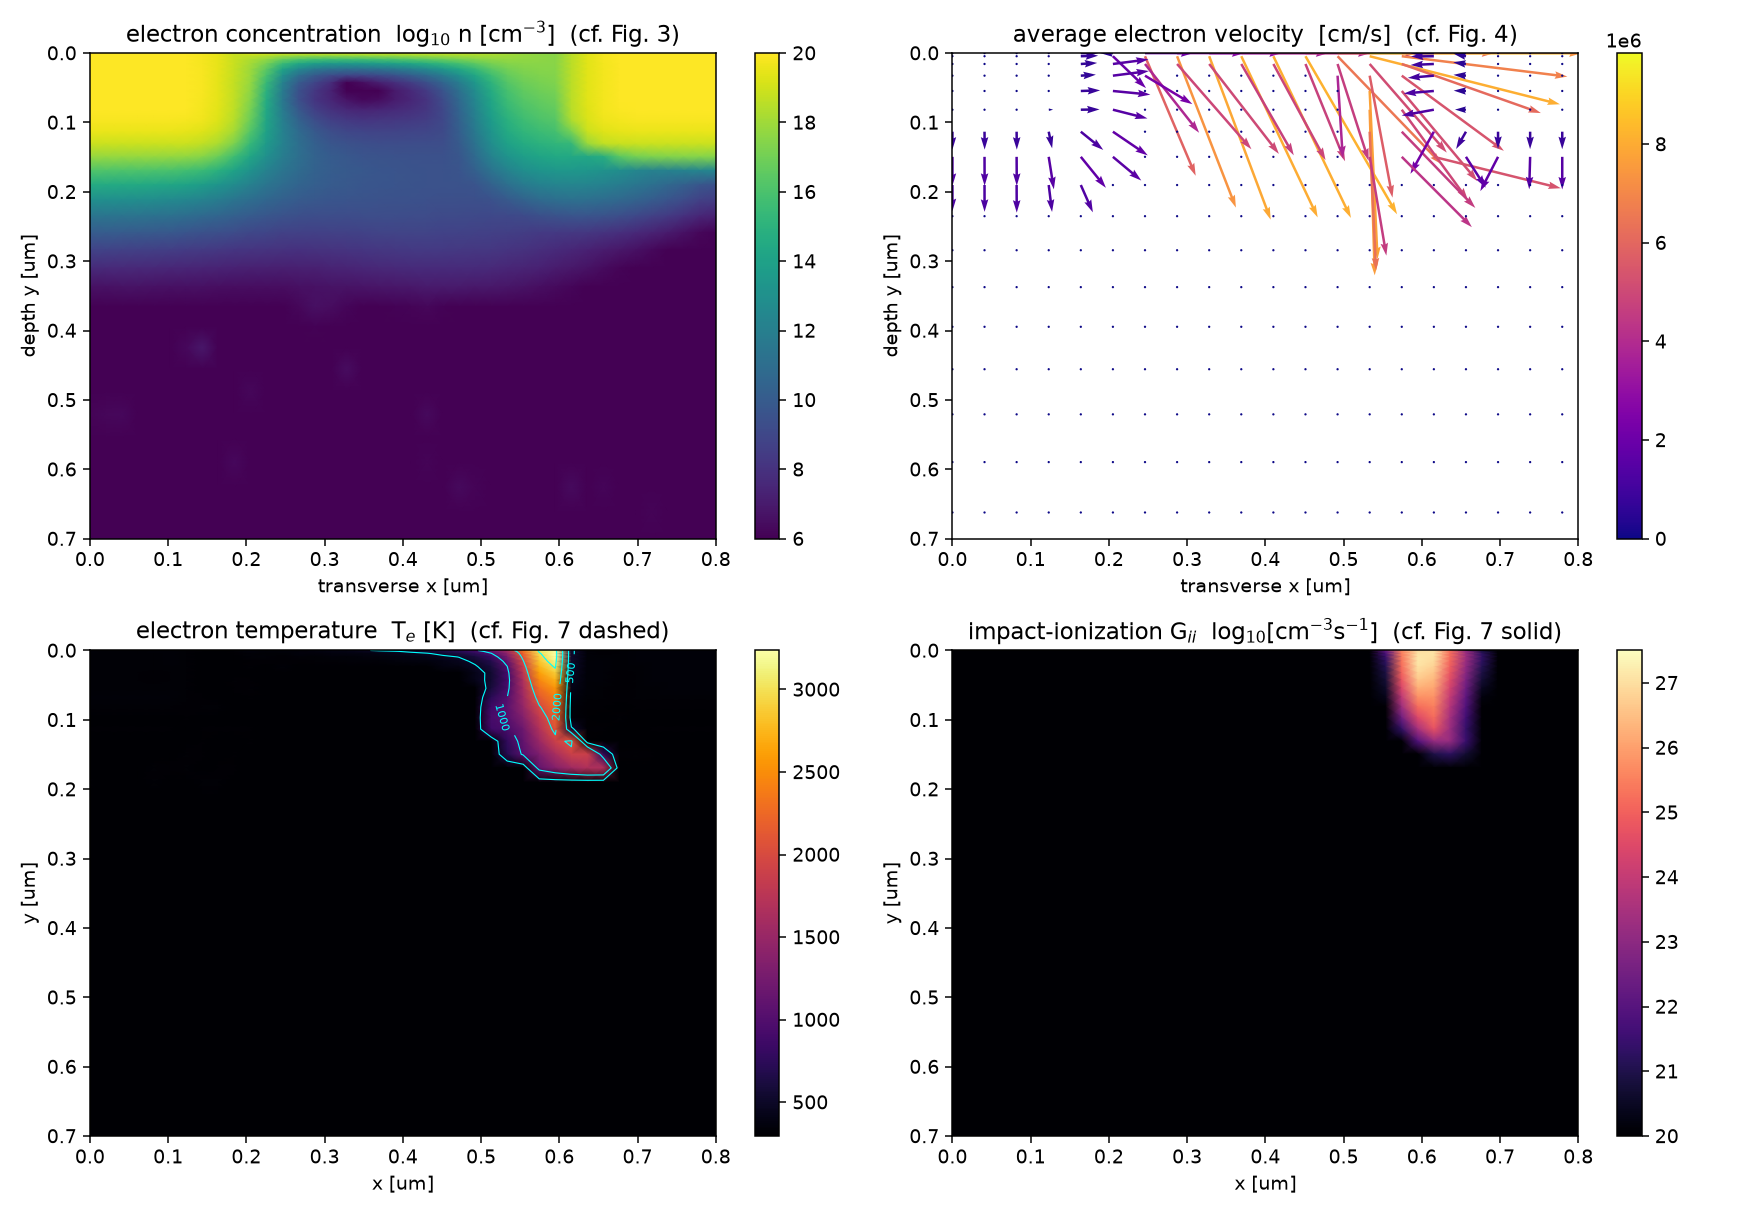
\includegraphics[width=\linewidth]{../figures/she2d_moments.png}
\caption{One-way SHE moments (40$\times$34). $n$ (Fig.~3), velocity field saturating at
$9.73\times10^6\,\si{cm/s}$ (Fig.~4; masked where $n<10^{13}\,\si{cm^{-3}}$), $T_e$ (Fig.~7
dashed, drain-localized), $G_{ii}$ (Fig.~7 solid, drain-localized).}
\end{figure}

\section{Grid refinement (40$\times$34 vs 60$\times$50, one-way)}\label{sec:grid}
Refining the spatial mesh at fixed $\Delta H=\SI{12.5}{meV}$:
\begin{center}\small
\begin{tabular}{lrrl}
\toprule
Quantity & 40$\times$34 & 60$\times$50 & converged? \\
\midrule
$n_{\max}$ & $1.0516\times10^{20}$ & $1.0473\times10^{20}$ & yes ($-0.4\%$) \\
$|v|_{\max}$ & $9.73\times10^{6}$ & $10.0\times10^{6}$ & yes ($+2.7\%$) \\
$T_{e,\max}$ [K] & $3232.9$ & $3423.0$ & moderate ($+5.9\%$) \\
$G_{ii,\max}$ & $1.3513\times10^{27}$ & $8.26\times10^{26}$ & \textbf{no} ($-40\%$) \\
$T_e$/$G_{ii}$ separation & 1 cell & 2 cells & grid-scale (unresolved) \\
current mismatch / residual & 0.16\% / $5.7\!\times\!10^{-6}$ & 0.07\% / $7.6\!\times\!10^{-6}$ & conserved \\
\bottomrule
\end{tabular}
\end{center}
$n$ and $|v|$ are spatially robust over this refinement; $T_e$ is moderately grid-sensitive
($5.9\%$, not converged); $G_{ii}$ is \emph{not} grid-converged (it
depends on the high-energy tail); and the peak separation tracks the mesh, so it is unresolved,
not a reproduced physical offset.

\section{Self-consistent SHE$\leftrightarrow$Poisson$\leftrightarrow$hole loop}\label{sec:coupled}
A damped outer iteration solves the SHE (with impact ionization) on the current potential, drives
hole continuity with $G_{ii}$ as pair generation (holding $n_{\text{SHE}}$), updates Poisson from
the SHE density, damps, and repeats; $n$ is recomputed from the SHE after each potential update
(not constitutively from DD). Over 12 iterations (Fig.~\ref{fig:coupled}) the maximum potential
update falls monotonically $17.7\to\SI{4.0}{mV}$ and the observables \emph{appear} to plateau:
$G_{ii,\max}$ suppressed $37\%$ ($1.35\to0.85\times10^{27}$), drain current $29\%$
($1.71\to1.21\times10^{-4}\,$A/\si{\micro\meter}), $T_{e,\max}\sim\!\SI{3240}{K}$.
\textbf{This early plateau is only apparent}: extended to 50 iterations the \emph{damped Picard}
loop keeps drifting and never settles $G_{ii}$ (Fig.~\ref{fig:conv50}). The suppression itself is the
physically expected negative feedback --- the SHE electrons and the $G_{ii}$-generated holes reshape
the potential, lowering the peak drain field and throttling avalanche --- but \emph{converging} it
requires a better fixed-point solver than damped Picard: \S\ref{sec:giiconv} shows a stagnation-restart
Anderson acceleration \emph{does} reach the fixed point, at which $G_{ii}$ plateaus. Final
conservation is clean (relative number balance $2.4\times10^{-5}$, currents balance $0.14\%$).
\honest{Fig.~\ref{fig:coupled} is a 12-iteration Picard \emph{snapshot} whose apparent $G_{ii}$
plateau does \emph{not} survive --- damped Picard is simply too slow to reach the fixed point
(\S\ref{sec:giiconv}). The converged loop, and the converged $G_{ii}$, come from the
stagnation-restart Anderson solver, not from this Picard run.}

\begin{figure}[h]\centering
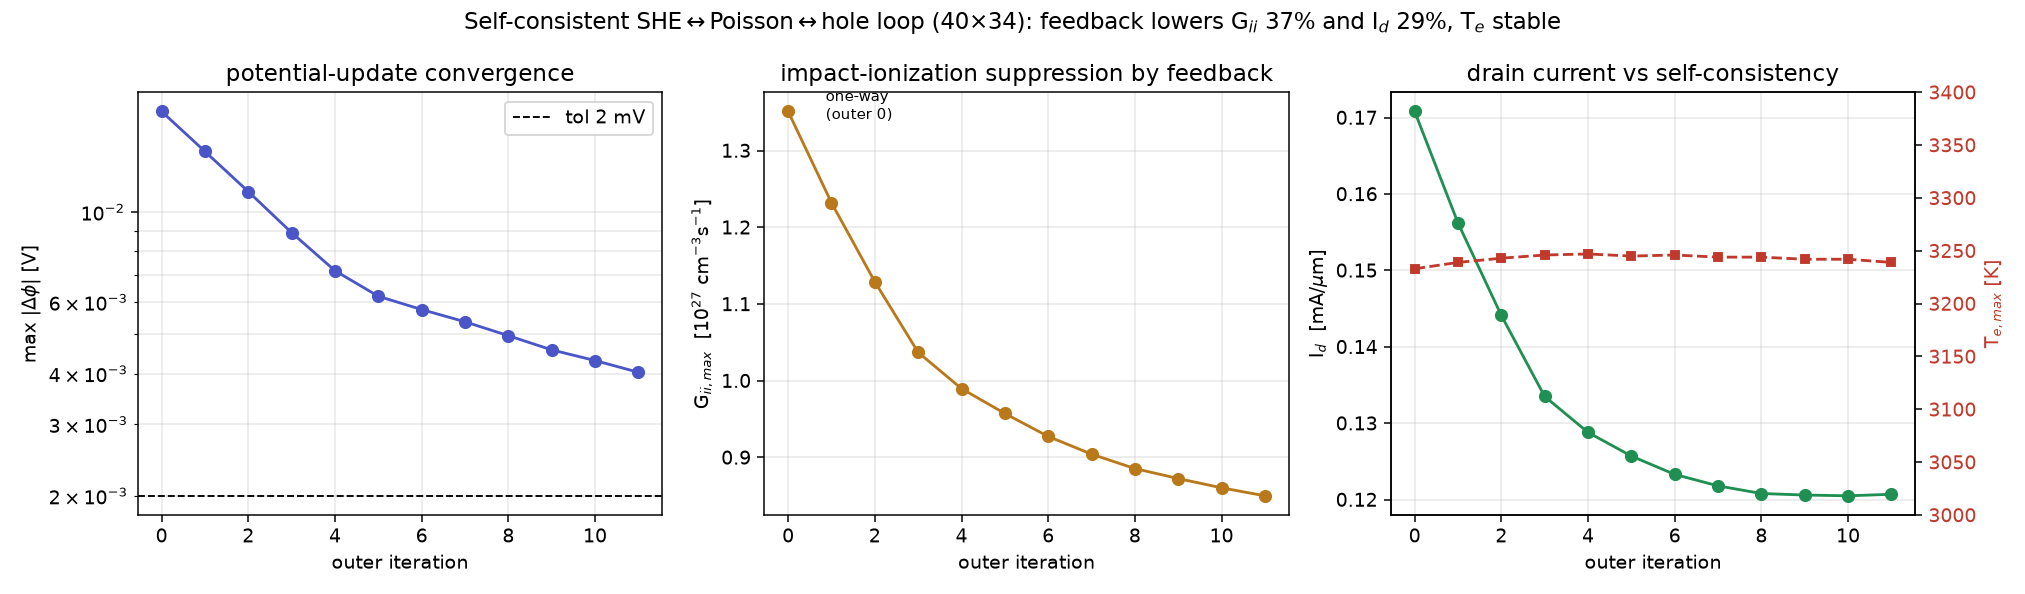
\includegraphics[width=\linewidth]{../figures/she2d_coupled_convergence.png}
\caption{Self-consistent loop (40$\times$34), first 12 \emph{damped-Picard} iterations. Potential
update $17.7\to\SI{4.0}{mV}$; feedback suppresses $G_{ii}$ and $I_d$ with an \emph{apparent} early
plateau that does not survive (Picard stalls, Fig.~\ref{fig:conv50}); the converged loop uses the
stagnation-restart Anderson solver (\S\ref{sec:giiconv}, Fig.~\ref{fig:anderson}).}
\label{fig:coupled}
\end{figure}

\section{$G_{ii}$ convergence matrix and device recalibration}\label{sec:giiconv}
Combining one-way and \emph{converged} coupled runs at both grids isolates how the impact-ionization
magnitude responds to spatial refinement and to self-consistency (Table~\ref{tab:giimat}). With the
stagnation-restart Anderson solver (below) the coupled column now holds true fixed-point values, not
the under-converged Picard snapshots of earlier revisions. Two facts emerge. \emph{(i)~Feedback is
strong and now converged:} the coupled $G_{ii,\max}$ is $-84\%$ (40$\times$34) and $-89\%$
(60$\times$50) below the one-way value on the same recalibrated potential --- a much larger, and
finally \emph{settled}, suppression than the $-37$--$53\%$ under-converged snapshots quoted before.
\emph{(ii)~The converged $G_{ii}$ is strongly mesh-dependent:} $-69\%$ from 40$\times$34 to
60$\times$50, exceeding even the one-way spatial drop ($-54\%$) because the feedback amplifies the
grid-dependence of the drain hotspot. The earlier ``multiplicatively separable to $\sim$1\%''
relation was an artifact of the matched \emph{under-converged} snapshots; it does not hold for the
converged fields, and no simple separable scaling is claimed. Because the converged coupled value
still moves $-69\%$ under the one spatial refinement tested, \emph{no continuum $G_{ii}$ can be
quoted}: the fixed point is now controlled, but the mesh is not.

\begin{table}[h]\centering\small
\caption{$G_{ii,\max}$ [\si{cm^{-3}s^{-1}}] over grid $\times$ coupling (recalibrated device,
$\Phi_{gate}=\SI{-0.74}{V}$). The coupled column holds \emph{converged} fixed-point values
(stagnation-restart Anderson, Fig.~\ref{fig:anderson}); the one-way column is iteration~0 of the same
loop (SHE on the recalibrated DD potential). Both fall with refinement; the converged coupled value
is $-69\%$ from 40$\times$34 to 60$\times$50.}\label{tab:giimat}
\begin{tabular}{lrr}
\toprule
 & one-way (iter 0) & coupled (converged) \\
\midrule
40$\times$34 & $4.61\times10^{27}$ & $7.44\times10^{26}$ \\
60$\times$50 & $2.12\times10^{27}$ & $\mathbf{2.29\times10^{26}}$ \\
\bottomrule
\end{tabular}
\end{table}

A \emph{one-way} energy refinement to $\Delta H=\SI{6.25}{meV}$ ($E_{op}=8$) moves $G_{ii,\max}$
only $-2.4\%$ ($T_e$ $-0.19\%$) --- \emph{negligible beside} the $-69\%$ spatial change --- so the
dominant numerical uncertainty is resolving the drain-side high-field/high-energy hotspot in real
space, not the energy axis. (The energy test was performed one-way, so we state energy
insensitivity, not a proof of purely-spatial error.) $2.29\times10^{26}$ is thus the
\emph{finest-tested converged coupled value}, not an estimate of the continuum limit: with a $-69\%$
change under the last spatial refinement there is no basis to quote a mesh-converged $G_{ii}$. The
mesh-robust results are $n$, $|v|$ and the terminal current $I_d$ ($+3\%$ over the refinement); the
feedback suppression is now converged \emph{per grid} ($-84$/$-89\%$) but is itself grid-dependent.

\paragraph{Device recalibration and the converged coupled loop.} A rigid gate offset
$\Phi_{gate}=\SI{-0.74}{V}$ ($dV_{th}/d\Phi_{gate}\!\approx\!+1$) recalibrates the extracted
threshold to $V_{th}=\SI{0.614}{V}$ (was \SI{1.64}{V}); the $V_g=\SI{3}{V}$ overdrive becomes
\SI{2.39}{V}. On this device the \emph{damped Picard} loop does not converge $G_{ii}$: over 50
iterations $\max|\Delta\phi|$ only reaches \SI{2.5}{mV} and $G_{ii,\max}$ drifts monotonically
$2.1\times10^{27}\to6.3\times10^{26}$, still falling (Fig.~\ref{fig:conv50}) --- the earlier
``$G_{ii}$ does not converge in the loop'' conclusion. \textbf{That was a solver limitation, not
physics.} A stagnation-restart Anderson acceleration (Fig.~\ref{fig:anderson}) --- least-squares
mixing on the free potential DOFs, with the difference history flushed whenever the residual stalls
and the least-squares regularized ($\mathrm{rcond}=10^{-8}$) --- reaches the fixed point at both
grids. $G_{ii,\max}$ \emph{plateaus}: $7.44\times10^{26}$ at 40$\times$34 (last-4 spread $0.33\%$)
and $2.29\times10^{26}$ at 60$\times$50 ($0.21\%$), with $T_{e,\max}$ ($2734$/\SI{3092}{K}),
$n_{\max}\approx1.0\times10^{20}$ and $I_d$ ($0.29$/\SI{0.30}{mA/\micro\meter}) all flat. The
max-norm potential residual floors at $0.6$--\SI{1.5}{mV} --- a handful of drain-hotspot nodes
wiggling below the observables' convergence, so it does not reach the strict \SI{1e-4}{V} tolerance,
yet every physical moment is settled to $<0.5\%$. The recalibrated Picard snapshot
$1.34\times10^{27}$ and the falling Picard $6.3\times10^{26}$ were both far from this converged
$2.29\times10^{26}$. The overlays of \S\ref{sec:compare} use the \emph{converged} 60$\times$50
fields, on which $T_e$ reaches $62\%$ and $G_{ii}$ $10\%$ of Liang's top contours --- the latter now
a converged (if mesh-dependent) value, not a still-falling snapshot.

\begin{figure}[h]\centering
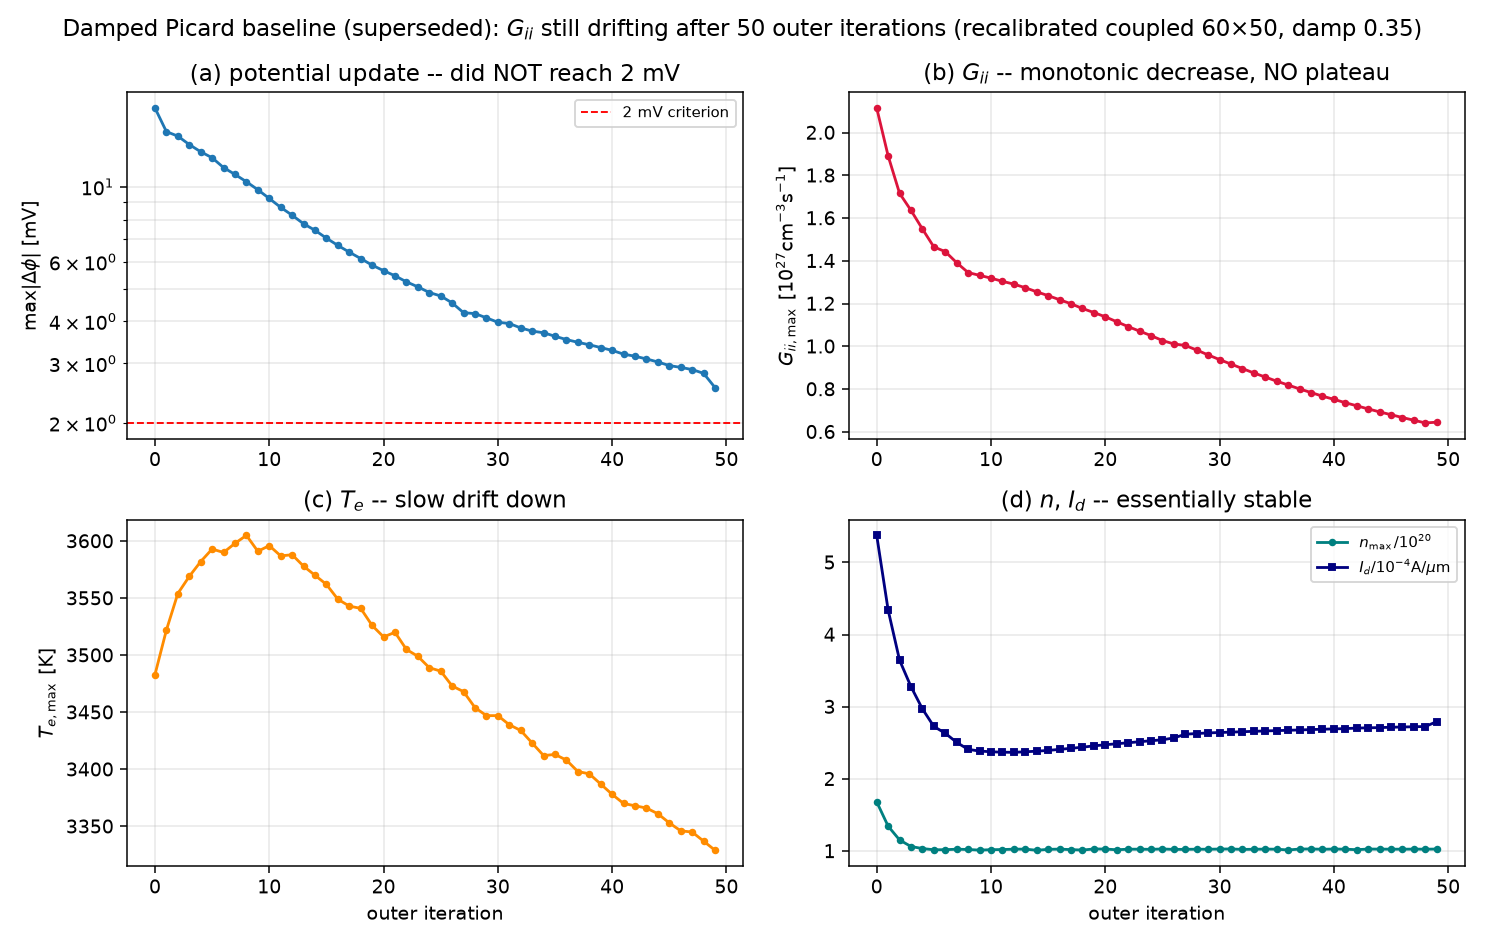
\includegraphics[width=\linewidth]{../figures/she2d_converge_60x50.png}
\caption{The \emph{damped-Picard} 60$\times$50 loop stalls (50 iterations, $\phi$-damping $0.35$):
(a) $\max|\Delta\phi|$ falls only to \SI{2.5}{mV}; (b) $G_{ii,\max}$ drifts monotonically with
\emph{no plateau}; (c) $T_e$ drifts down; (d) $n$, $I_d$ stable. This slow non-convergence motivated
the stagnation-restart Anderson solver (Fig.~\ref{fig:anderson}), which reaches the fixed point
Picard could not.}\label{fig:conv50}
\end{figure}

\begin{figure}[h]\centering
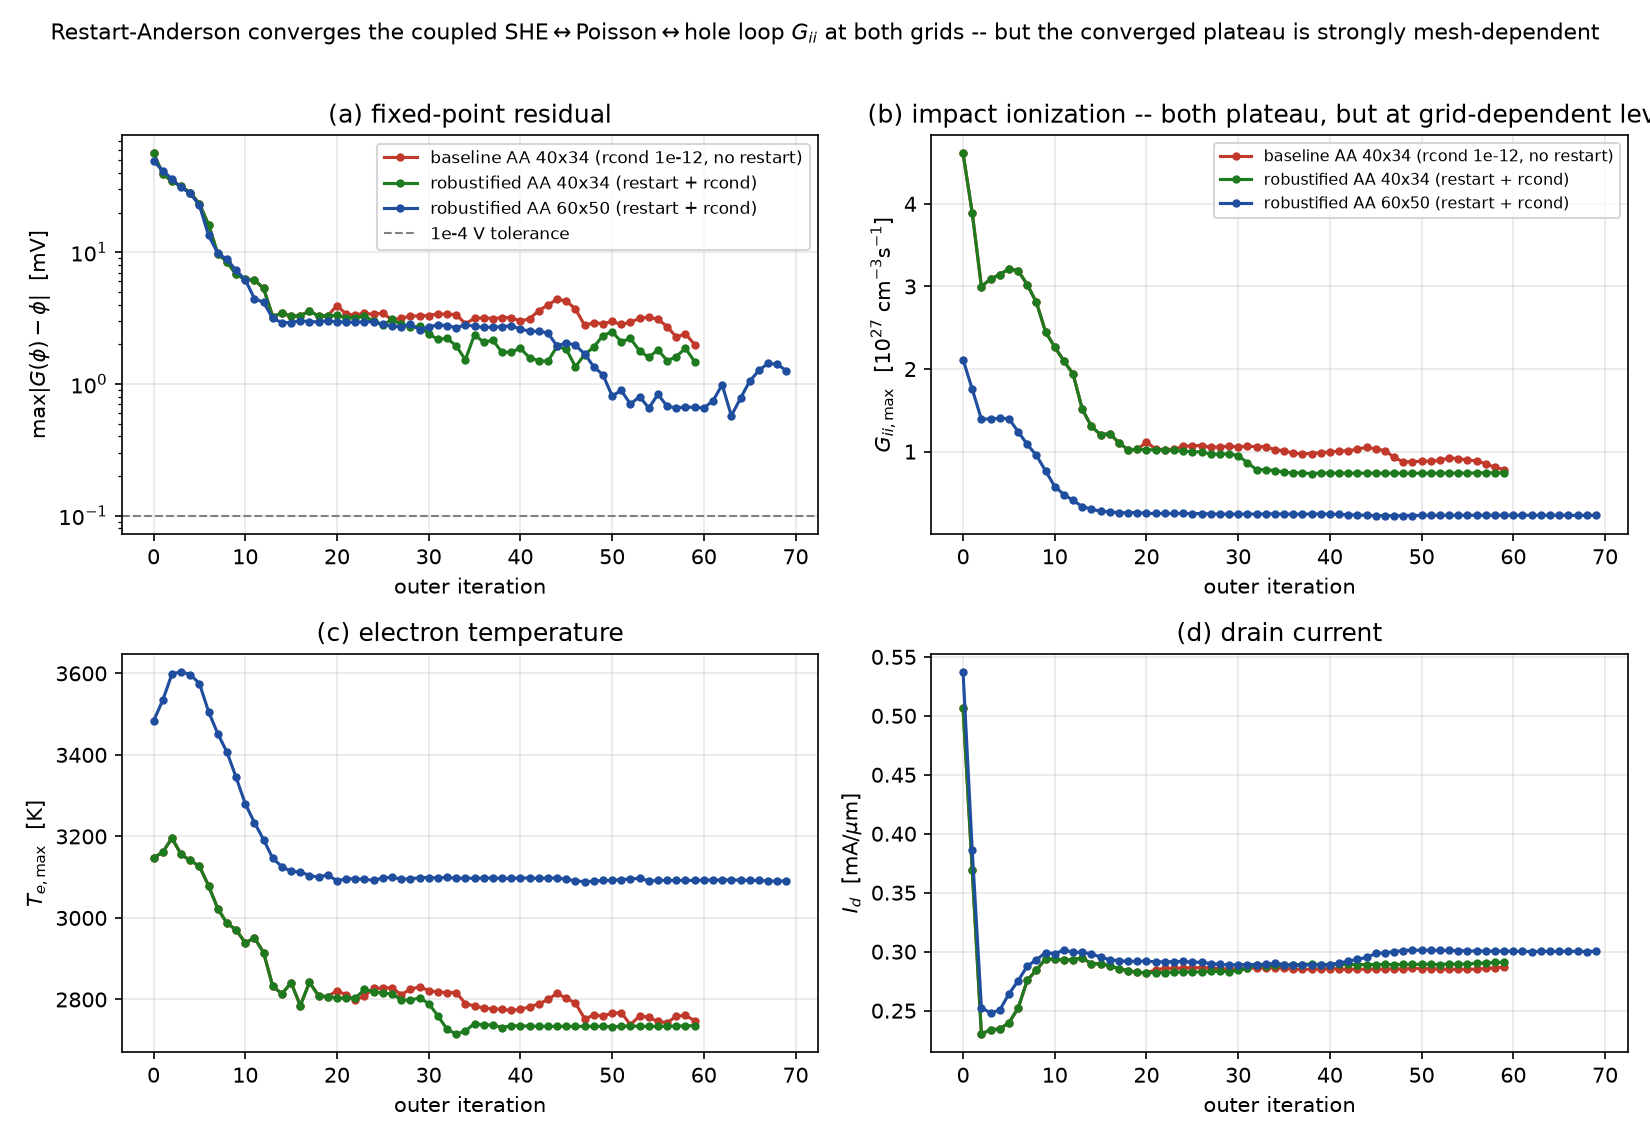
\includegraphics[width=\linewidth]{../figures/anderson_converge.png}
\caption{Stagnation-restart Anderson acceleration of the coupled loop. (a) fixed-point residual
$\max|G(\phi)-\phi|$; (b) $G_{ii,\max}$; (c) $T_{e,\max}$; (d) $I_d$. Baseline Anderson
(rcond~$10^{-12}$, no restart; red) stalls like Picard; the restart-plus-regularized solver
converges $G_{ii}$ to a flat plateau at 40$\times$34 (green, $7.44\times10^{26}$) and 60$\times$50
(blue, $2.29\times10^{26}$). Both grids plateau, but at strongly grid-dependent levels; $I_d$~(d) is
mesh-robust.}\label{fig:anderson}
\end{figure}

\section{Quantitative comparison with Liang's published figures}\label{sec:compare}
The \emph{converged} recalibrated coupled 60$\times$50 solution (\S\ref{sec:giiconv},
$V_{th}=\SI{0.614}{V}$) is compared to Liang \emph{et al.}'s figures below, with \emph{one comparison table per plot}
(Figs.~2--8, Tables~\ref{tab:f2}--\ref{tab:f8}). Where Liang give labelled contour values (Fig.~7)
the comparison is on those values; otherwise it is on peak magnitudes, locations, and structure.
Liang's Fig.~7 levels (paper caption, p.~263) are $T_e\in\{500,1000,2000,3000,4500,4800,5000\}$~K
(dashed) and $G_{ii}\in\{1.0,4.0\}\times10^{26},\{1.0,1.7,2.3\}\times10^{27}\,\si{cm^{-3}s^{-1}}$
(solid). (A Rev.~3 transcription that omitted the \SI{4800}{K} level and added a spurious
$2.3\times10^{26}$ $G_{ii}$ level was corrected in Rev.~4, and the overlays regenerated.)

\begin{figure}[h]\centering
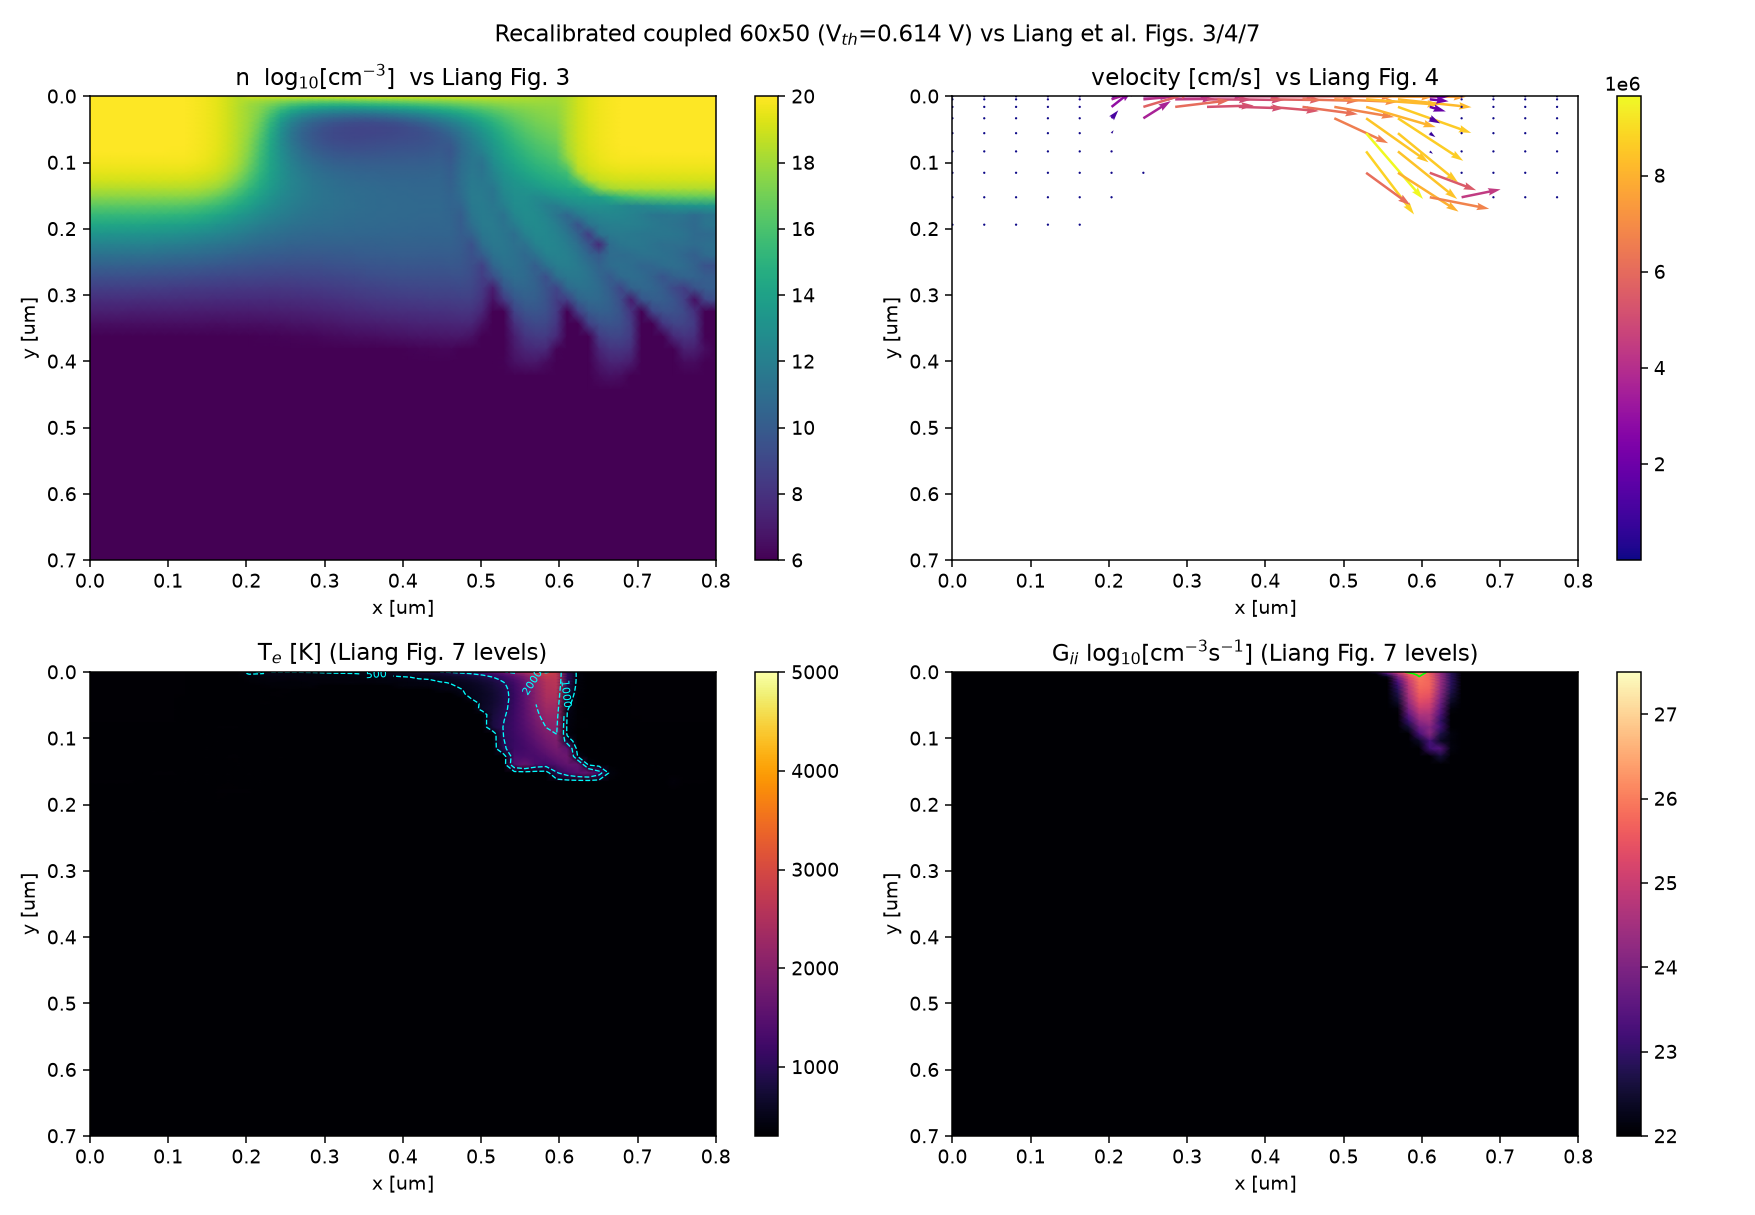
\includegraphics[width=\linewidth]{../figures/she2d_liang_compare.png}
\caption{This work vs Liang Figs.~3 ($n$), 4 (velocity), 7 ($T_e$, $G_{ii}$ at Liang's contour levels).}
\label{fig:cmp}
\end{figure}

\begin{figure}[h]\centering
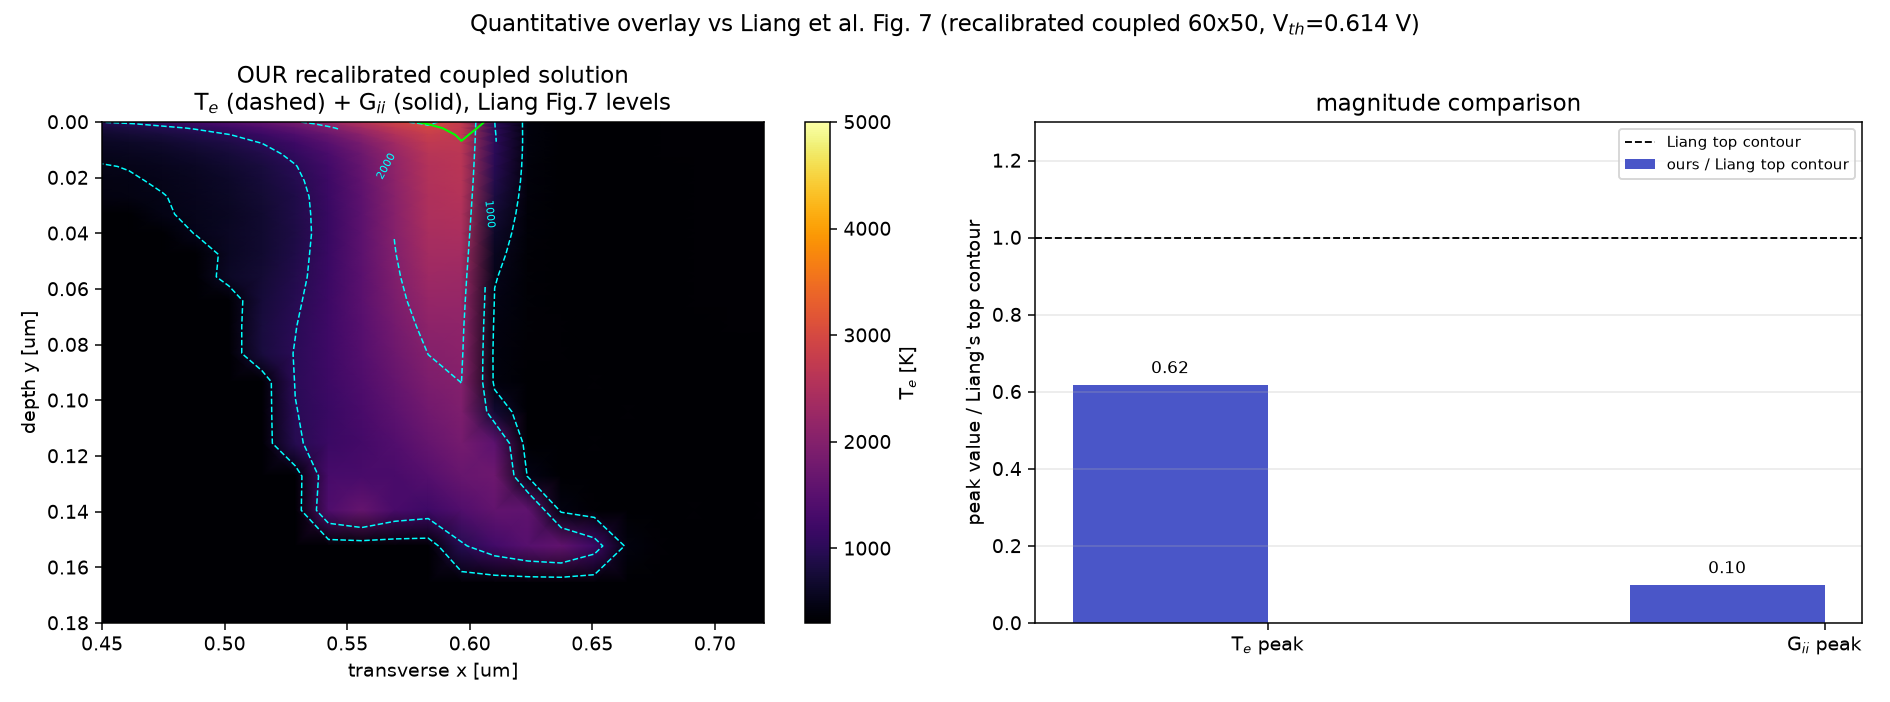
\includegraphics[width=0.86\linewidth]{../figures/she2d_liang_fig7_overlay.png}
\caption{Quantitative Liang Fig.~7 overlay: our $T_e$ (dashed) and $G_{ii}$ (solid) on Liang's exact
published levels; peaks reach $0.62$ ($T_e$) and $0.10$ ($G_{ii}$, mesh-unconverged) of the top contours.}
\label{fig:ov7}
\end{figure}

\begin{figure}[h]\centering
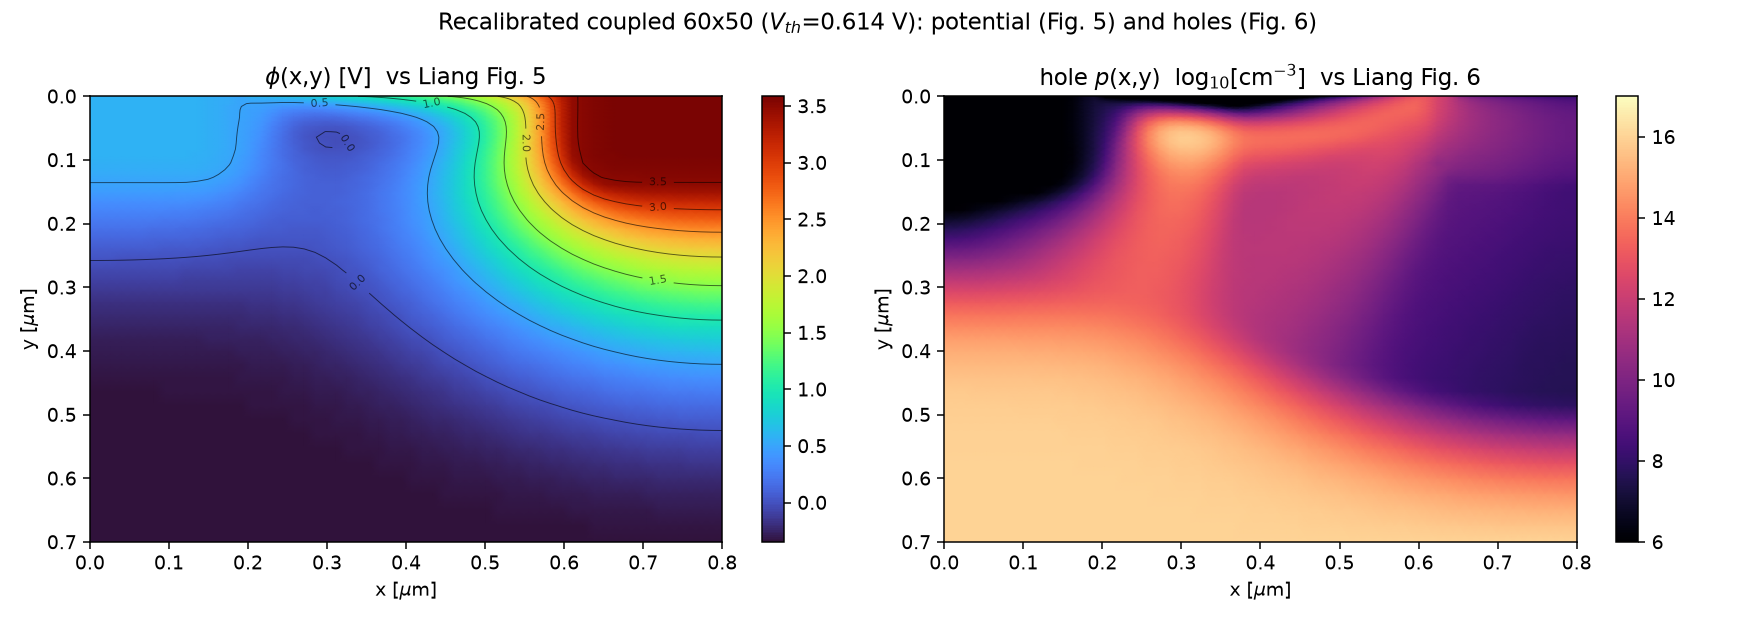
\includegraphics[width=\linewidth]{../figures/she2d_liang_fig5_6.png}
\caption{Potential $\phi$ (Liang Fig.~5) and hole concentration $p$ (Liang Fig.~6), recalibrated
coupled 60$\times$50: $\phi$ rises smoothly source$\to$drain; holes fill the p-body and are depleted
in the n$^+$ S/D.}\label{fig:pot}
\end{figure}

\begin{figure}[h]\centering
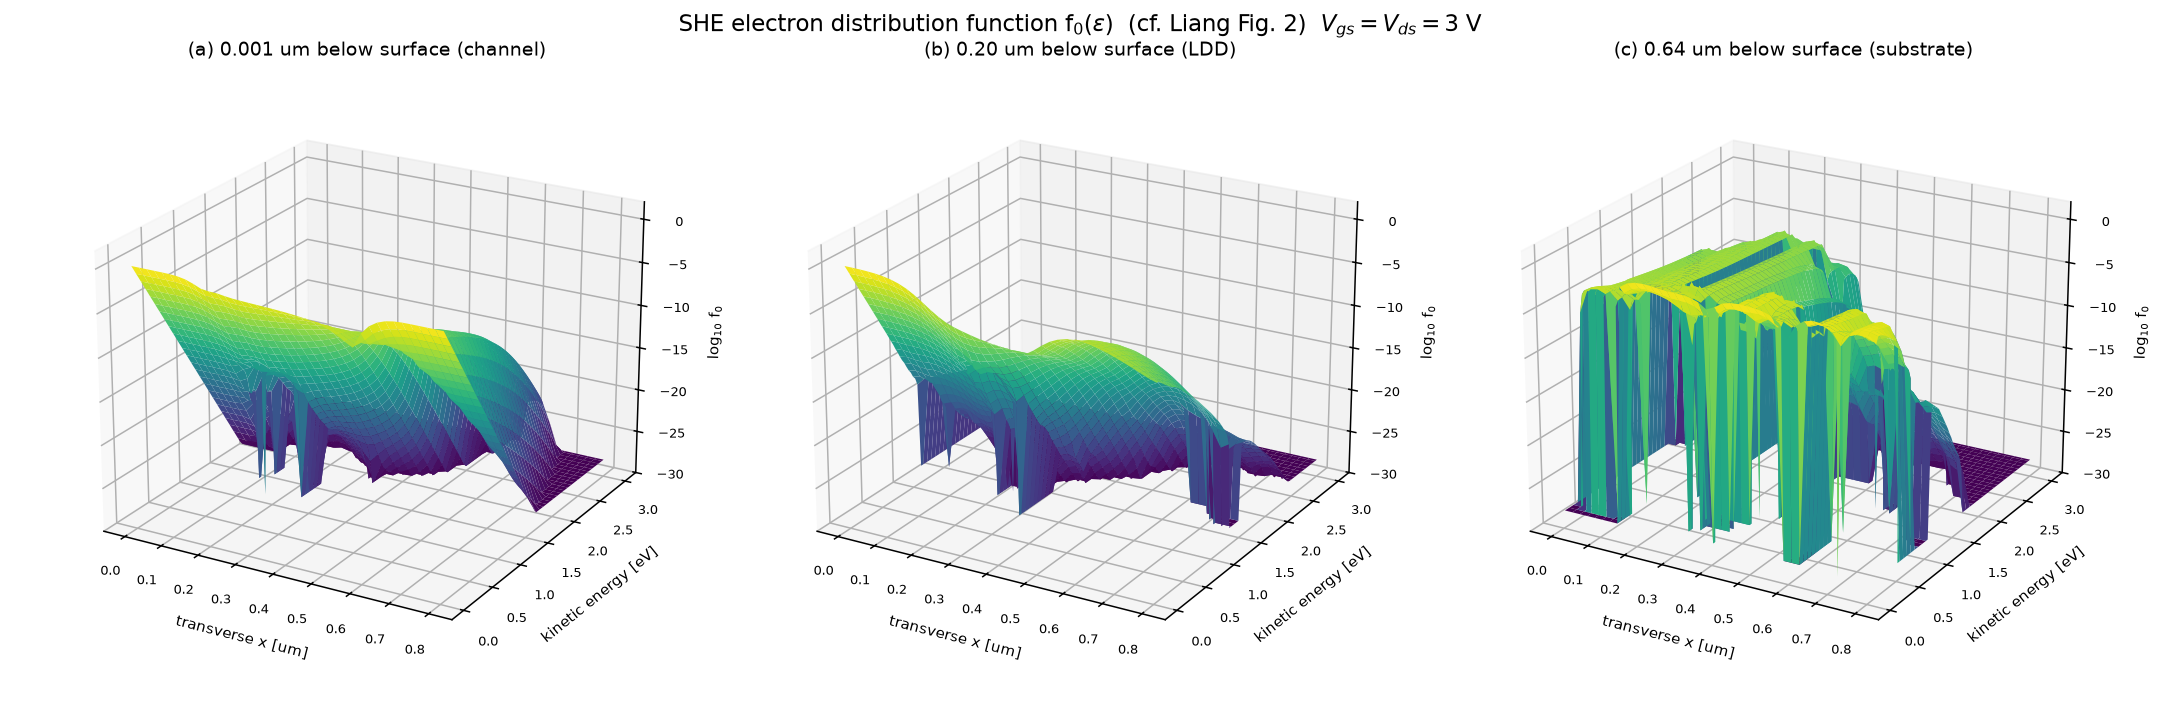
\includegraphics[width=0.82\linewidth]{../figures/she2d_fig2_distribution.png}
\caption{Energy distribution (Liang Fig.~2): a hot, non-Maxwellian tail localized at the drain
surface, thermal in the bulk.}\label{fig:dist}
\end{figure}

\begin{figure}[h]\centering
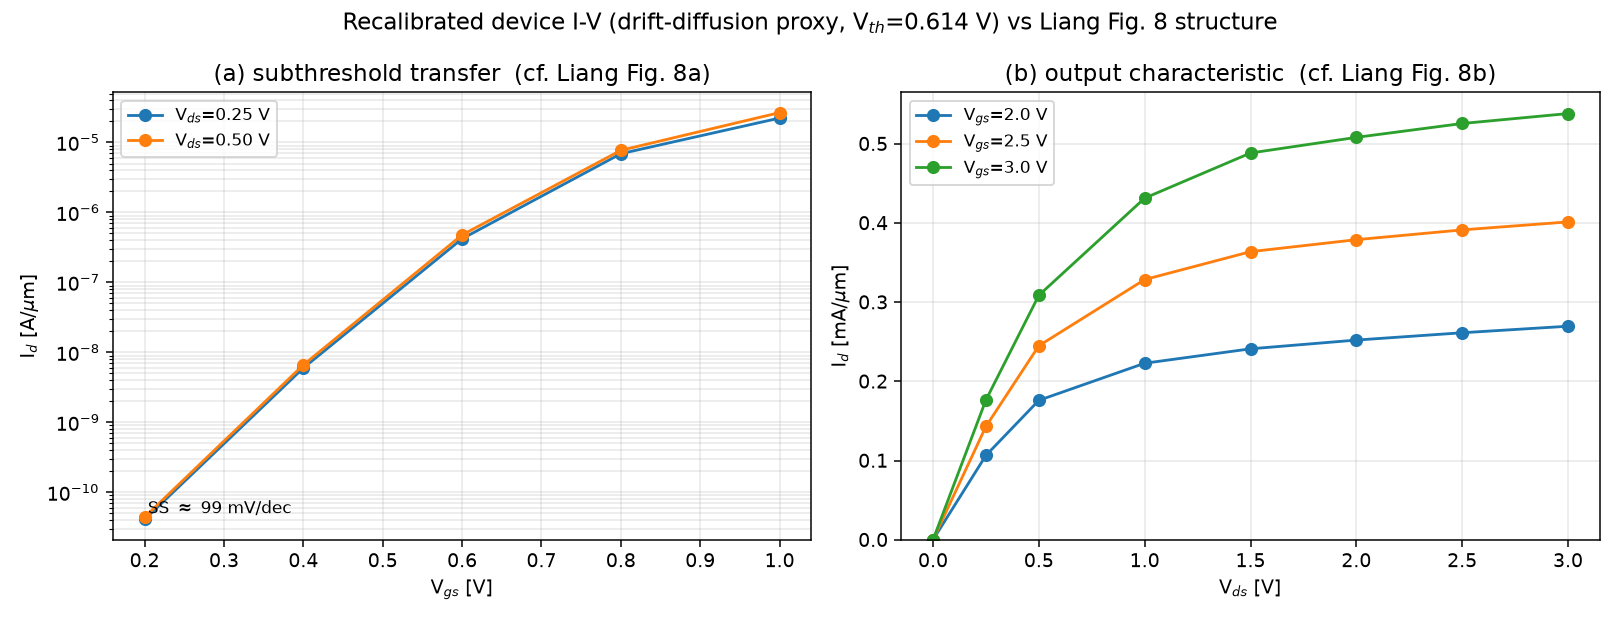
\includegraphics[width=\linewidth]{../figures/she2d_iv_fig8.png}
\caption{Terminal I-V (Liang Fig.~8), drift-diffusion proxy, per micron: (a) subthreshold transfer
at $V_{ds}=0.25,\SI{0.5}{V}$; (b) output characteristic at $V_{gs}=2.0,2.5,\SI{3.0}{V}$.}\label{fig:iv}
\end{figure}

\begin{figure}[h]\centering
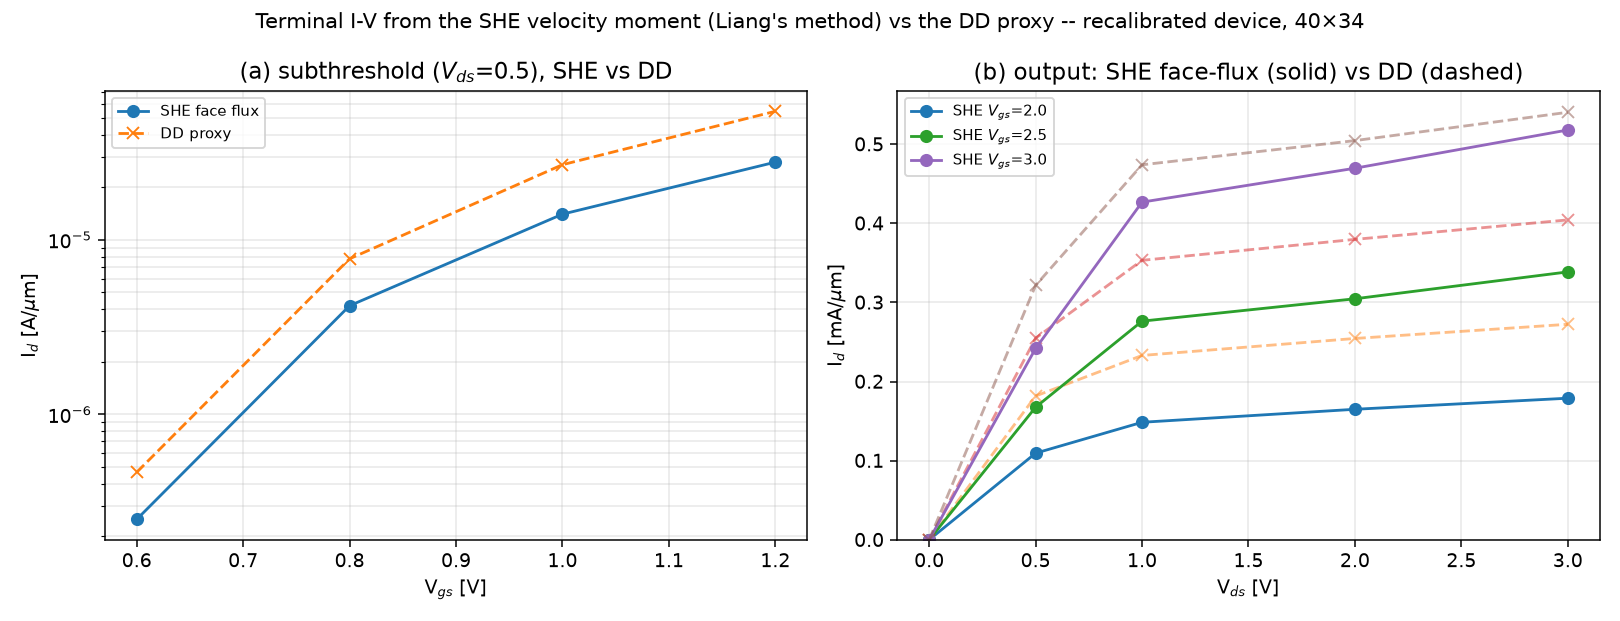
\includegraphics[width=\linewidth]{../figures/she2d_iv_moment.png}
\caption{Terminal I-V from the \emph{SHE velocity moment} (finite-volume face-flux current ---
Liang's method), one-way SHE on the DD potential, vs the DD proxy (dashed); recalibrated device,
40$\times$34. (a) subthreshold at $V_{ds}=\SI{0.5}{V}$ \emph{only} --- a partial reproduction of
Liang's Fig.~8(a), which also shows \SI{0.25}{V}; (b) output families
$V_{gs}=2.0,2.5,\SI{3.0}{V}$. Source/drain current conservation $|I_{src}{+}I_{drn}|/\overline{|I|}$
is $2\times10^{-5}$--$10^{-3}$ across the sweep (largest at $V_{ds}=\SI{3}{V}$), so the reported
current is the genuine SHE terminal flux. The \emph{measured} ratio $I_{d,\text{SHE}}/I_{d,\text{DD}}$
is $0.51$--$0.54$ (subthreshold) and $0.60$--$0.96$ (output, rising toward unity at high
$V_{gs}$/$V_{ds}$): the SHE current is systematically below the mobility-based DD proxy, consistent
with the stronger nonlocal/high-field transport in the SHE solution (not attributed to a single
mechanism absent a controlled diagnostic).}\label{fig:ivmoment}
\end{figure}

\clearpage
\noindent Per-plot comparison tables (columns: feature / this work / Liang / assessment).

\begin{table}[h]\centering\small
\caption{Liang Fig.~2 --- carrier energy distribution / hot electrons (this work: Fig.~\ref{fig:dist}).}\label{tab:f2}
\begin{tabular}{p{3.5cm}p{3.9cm}p{2.9cm}p{3.2cm}}
\toprule
Feature & This work & Liang & Assessment \\
\midrule
Drain-surface $T_e$ (tail temp.) & 3300--3600 K & hot, non-Maxwellian tail & hot tail reproduced \\
Source / bulk $T_e$ & 300--330 K & thermal & thermal, matches \\
High-energy tail cutoff & $\eps_{max}=\SI{3.02}{eV}$ (absorbing) & tail to high $\eps$ & bounded tail \\
Localization & drain-surface hot spot & near-drain surface & match \\
\bottomrule
\end{tabular}
\end{table}

\begin{table}[h]\centering\small
\caption{Liang Fig.~3 --- electron concentration $n(x,y)$ (this work: Fig.~\ref{fig:cmp}).}\label{tab:f3}
\begin{tabular}{p{3.5cm}p{3.9cm}p{2.9cm}p{3.2cm}}
\toprule
Feature & This work & Liang & Assessment \\
\midrule
$n_{\max}$ (S/D) & $1.02\times10^{20}\,\si{cm^{-3}}$ @ (0.10,\,0.02) & $\sim\!10^{20}$ & match \\
Channel inversion (surface) & $3.1\times10^{19}\,\si{cm^{-3}}$ & inversion layer & match \\
Drain pinch-off & $n$ decreases toward drain & pinch-off & match \\
\bottomrule
\end{tabular}
\end{table}

\begin{table}[h]\centering\small
\caption{Liang Fig.~4 --- average electron velocity (this work: Fig.~\ref{fig:cmp}).}\label{tab:f4}
\begin{tabular}{p{3.5cm}p{3.9cm}p{2.9cm}p{3.2cm}}
\toprule
Feature & This work & Liang & Assessment \\
\midrule
$|v|_{\max}$ & $9.9\times10^{6}\,\si{cm/s}$ @ drain & $\sim\!10^{7}$ (sat.) & match \\
Field pattern & lateral in channel, downward into drain & source$\to$drain, into drain & match \\
Saturation & velocity-saturated near drain & yes & match \\
\bottomrule
\end{tabular}
\end{table}

\begin{table}[h]\centering\small
\caption{Liang Fig.~5 --- electrostatic potential $\phi(x,y)$ (this work: Fig.~\ref{fig:pot}).}\label{tab:f5}
\begin{tabular}{p{3.5cm}p{3.9cm}p{2.9cm}p{3.2cm}}
\toprule
Feature & This work & Liang & Assessment \\
\midrule
$\phi$ swing & $-0.35\to+3.59$~V (3.93~V) & $V_{ds}$=3 + built-ins & match \\
Source-surface $\phi$ & \SI{0.59}{V} (built-in) & built-in & match \\
Drain-surface $\phi$ & \SI{3.59}{V} ($=V_{ds}+$built-in) & $\approx\!V_{ds}$ & match \\
Profile & smooth, monotone S$\to$D & smooth 2-D & structural (reconstr.\ doping) \\
\bottomrule
\end{tabular}
\end{table}

\begin{table}[h]\centering\small
\caption{Liang Fig.~6 --- hole concentration $p(x,y)$ (this work: Fig.~\ref{fig:pot}).}\label{tab:f6}
\begin{tabular}{p{3.5cm}p{3.9cm}p{2.9cm}p{3.2cm}}
\toprule
Feature & This work & Liang & Assessment \\
\midrule
$p_{\max}$ & $2.1\times10^{16}\,\si{cm^{-3}}$ (p-body) & p-body / substrate & match (structural) \\
n$^+$ S/D holes & $\le\!4\times10^{13}\,\si{cm^{-3}}$ (depleted) & hole-depleted & match \\
II holes near drain & elevated $p$ from $G_{ii}$ source & avalanche holes & present \\
Caveat & body-contact BC + reconstr.\ doping & --- & structural, not point-wise \\
\bottomrule
\end{tabular}
\end{table}

\begin{table}[h]\centering\small
\caption{Liang Fig.~7 --- $T_e$ (dashed) and $G_{ii}$ (solid) contours (this work: Figs.~\ref{fig:cmp},\ref{fig:ov7}).}\label{tab:f7}
\begin{tabular}{p{3.5cm}p{3.9cm}p{2.9cm}p{3.2cm}}
\toprule
Feature & This work & Liang & Assessment \\
\midrule
$T_{e,\max}$ & \SI{3092}{K} (62\% of top) & to \SI{5000}{K} & same order, drain-localized \\
$G_{ii,\max}$ & $2.29\times10^{26}$ (10\% of top) & to $2.3\times10^{27}$ & loop-converged; mesh-unconverged ($-69\%$) \\
$T_e$ vs $G_{ii}$ extent & $T_e$ region $\sim\!30\times$ larger & $T_e$ broader & match \\
Peak offset & $\le\!1$ cell (14~nm) & offset & unresolved at mesh \\
\bottomrule
\end{tabular}
\end{table}

\begin{table}[h]\centering\small
\caption{Liang Fig.~8 --- terminal I-V (this work: Figs.~\ref{fig:iv},\ref{fig:ivmoment}).}\label{tab:f8}
\begin{tabular}{p{3.3cm}p{4.4cm}p{2.5cm}p{3.1cm}}
\toprule
Feature & This work & Liang & Assessment \\
\midrule
I-V method & SHE velocity moment (face flux), one-way (Fig.~\ref{fig:ivmoment}) & BTE velocity moment & \emph{method reproduced} (one-way) \\
Output shape & triode$\to$sat, $V_{gs}$-ordered (SHE and DD) & Fig.~8b & shape match \\
$I_{d,\text{SHE}}(V_g{=}V_d{=}3)$ & \SI{0.52}{mA/\micro\meter} (SHE face flux) & --- & from BTE flux, not DD \\
$I_{d,\text{SHE}}/I_{d,\text{DD}}$ & 0.51--0.54 (sub.), 0.60--0.96 (out.) & --- & SHE below DD (measured) \\
S/D conservation & $2\times10^{-5}$--$10^{-3}$ & --- & genuine terminal flux \\
Subthreshold swing & $\sim$\SI{99}{mV/dec} (DD) & sub-$\mu$m NMOS & reasonable \\
\bottomrule
\end{tabular}
\end{table}

\honest{The comparisons apply \emph{our} model on Liang's \emph{levels}; they are not a pixel
registration. With a reconstructed doping profile the absolute spatial positions of the hotspots
need not coincide with Liang's, so structural agreement (drain-localization, $T_e$ broader than
$G_{ii}$, order-of-magnitude levels) is the claim, not point-by-point overlap. $G_{ii,\max}$ is now
\emph{loop-converged} but still mesh-unconverged (\S\ref{sec:giiconv}), so its 10\%-of-top value is a
converged-but-mesh-dependent figure ($-69\%$ under the last refinement), not a continuum bound; and
the $T_e$/$G_{ii}$ peak offset stays within one cell.
\textbf{The Fig.~8 I-V now includes a SHE velocity-moment current} (Fig.~\ref{fig:ivmoment}): the
terminal current is read from the SHE finite-volume face flux, reproducing Liang's method (current
from the BTE moment, \emph{not} a mobility model), with source/drain conservation
$2\times10^{-5}$--$10^{-3}$. It is \emph{one-way} (SHE on the DD potential, not the full coupled
loop), so it demonstrates the method but is not yet a self-consistent I-V. The DD proxy is retained
for comparison; the measured $I_{d,\text{SHE}}/I_{d,\text{DD}}=0.5$--$0.96$ (bias-dependent),
systematically below DD --- consistent with the stronger nonlocal/high-field transport in the SHE,
though not attributed to a single mechanism here. Liang's Fig.~8 solid lines are moreover
\emph{experimental} data for a real device of unstated width, so only the per-width shape is
comparable, not the absolute ampere magnitude.}

\part{Assessment}
\section{Conclusions, classified}\label{sec:concl}
\begin{itemize}[leftmargin=1.4em,itemsep=2pt]
\item \textbf{Scope --- reduced reproduction.} This reproduces the principal 2-D \emph{signatures}
(transport moments, hot-electron localization, avalanche feedback) with a P1/($\ell\le1$) SHE, but
is \emph{not} a full reproduction of Liang's simulator: the explicit surface-roughness,
surface-acoustic, and ionized-impurity operators are lumped into $\tau_1$
(Table~\ref{tab:physmatrix}), the band is a 1-parameter Kane surrogate, and the doping is
reconstructed. Defensible label: a \emph{reduced P1/SHE-Boltzmann reproduction of the principal
signatures}, using reconstructed device data and surrogate scattering/band models.
\item \textbf{Calibration vs.\ validation.} The overlay device is calibrated ($V_{th}$ fitted to
\SI{0.614}{V} via $\Phi_{gate}$; Table~\ref{tab:calib}); quantitative agreements are calibrated
comparisons, with $|v|_{\max}$, the $T_e$/$G_{ii}$ \emph{localization}, and subthreshold swing as
the independent checks.
\item \textbf{Core SHE transport} shows a clean grid-sensitivity hierarchy over the tested
40$\times$34$\to$60$\times$50 refinement: $n$ \emph{stable} ($0.4\%$), $|v|$ \emph{stable}
($2.7\%$) and $I_d$ \emph{stable} ($3\%$); $T_e$ moderately sensitive ($5.9\%$; stable, not
converged); $G_{ii}$ \emph{strongly mesh-dependent} ($-69\%$ coupled, $-54\%$ one-way). ``Stable
over the tested refinement'' is a two-grid statement, not a proof of asymptotic convergence.
\item \textbf{Impact ionization:} now part of the assembled electron collision operator, with
explicit primary depletion and secondary redistribution ($G_{ii}$ is a moment of the II-affected
$f_0$); the equal-energy secondary split and negligible scattering-in shape change follow the
paper.
\item \textbf{Self-consistency:} the SHE$\leftrightarrow$Poisson$\leftrightarrow$hole feedback is
implemented and \emph{converges}. The damped Picard loop stalled (\SI{2.5}{mV} in 50 iterations,
$G_{ii}$ still drifting, Fig.~\ref{fig:conv50}), but a \emph{stagnation-restart Anderson}
acceleration (Fig.~\ref{fig:anderson}) reaches the fixed point at both grids: $G_{ii,\max}$ plateaus
($7.44\times10^{26}$ at 40$\times$34, $2.29\times10^{26}$ at 60$\times$50, last-4 spread
$\le0.33\%$), with $T_e$, $n$, $I_d$ flat. The earlier ``does not converge in the loop'' was a
\emph{solver artifact}; the converged feedback suppression is $-84$/$-89\%$ (vs.\ the superseded
$-37$/$-53\%$ snapshots).
\item \textbf{Quantitative overlays (this revision):} on Liang's own Fig.~7 contour levels the
\emph{converged} coupled 60$\times$50 fields reach 62\% ($T_e$) and 10\% ($G_{ii}$, converged but
mesh-dependent) of the top published contours, drain-localized and correctly structured ($T_e$
region much broader than $G_{ii}$); a one-way SHE velocity-moment I-V reproduces Liang's
current-extraction method (Fig.~\ref{fig:ivmoment}), with the DD curve retained for comparison. A
per-plot comparison table is given for each of Liang's Figs.~2--8 (\S\ref{sec:compare},
Tables~\ref{tab:f2}--\ref{tab:f8}).
\item \textbf{Conservation:} validated across one-way, refined, and coupled calculations
(number balance $10^{-5}$--$10^{-7}$; terminal currents balance $<0.2\%$).
\item \textbf{Numerics:} physics-split preconditioning removes the previous practical solver
bottleneck.
\item \textbf{$G_{ii}$:} the earlier $1.37\times10^{27}$ agreement with Liang was
\emph{demonstrably accidental} --- both spatial refinement and self-consistency push $G_{ii}$
downward. With the loop now converged (stagnation-restart Anderson) the coupled $G_{ii,\max}$ is a
well-defined fixed point at each grid --- $7.44\times10^{26}$ (40$\times$34) and $2.29\times10^{26}$
(60$\times$50) --- but it is \emph{strongly mesh-dependent} ($-69\%$ under the one refinement tested,
versus $-2.4\%$ for an energy refinement), so \emph{no continuum magnitude can be quoted}
(Table~\ref{tab:giimat}). The earlier ``the loop does not converge $G_{ii}$'' is retracted: that was
damped-Picard stagnation, and the under-converged snapshots ($1.34$/$5.24$/$6.3\times10^{26}$) are
all superseded by the converged values.
\item \textbf{$T_e$/$G_{ii}$ offset:} unresolved at present mesh resolution; \emph{no longer
claimed reproduced}.
\item \textbf{Device:} recalibrated to $V_{th}=\SI{0.614}{V}$ ($\Phi_{gate}=\SI{-0.74}{V}$),
replacing the earlier over-high \SI{1.64}{V}.
\item \textbf{Done this revision:} a one-way \emph{SHE velocity-moment} terminal I-V
(Fig.~\ref{fig:ivmoment}, Table~\ref{tab:f8}) --- terminal current from the SHE face flux, as in
Liang, with source/drain conservation $\le10^{-3}$ --- upgrading Fig.~8 from a DD shape check to a
demonstrated (if not yet self-consistent) reproduction of Liang's I-V method.
\item \textbf{Open items, in priority order.} (a) \emph{done} --- the accelerated coupled solver
(stagnation-restart Anderson) now converges the loop $G_{ii}$ at both grids (\S\ref{sec:giiconv}),
retiring the former ``fundamental blocker.'' The blocker is now \emph{spatial}: (b) a third (and
finer) grid to bound the continuum $G_{ii}$, since the converged coupled value still moves $-69\%$
under the one refinement tested and drain-local refinement is likely needed, plus
$\eps_{max}$/coupled-$\Delta H$ sensitivity on the converged state; (c) a fully self-consistent (not
one-way) SHE-moment I-V; (d) explicit surface-roughness / -acoustic / impurity operators replacing
the lumped $\tau_1$.
\end{itemize}

\appendix
\section{Reproducibility package}\label{sec:specs}
All values below are the literal code constants (\texttt{src/device.py}, \texttt{constants.py},
\texttt{she2d.py}, \texttt{dd.py}); the simulation is fully specified by them plus the run commands.

\paragraph{Constants.} $T=\SI{300}{K}$; $\eps_{Si}=11.7$, $\eps_{ox}=3.9$;
$n_i=1.45\times10^{10}\,\si{cm^{-3}}$; $m^*=0.32\,m_0$; $g_v=6$; $\alpha=\SI{0.5}{eV^{-1}}$.
Table~I: $D_{ac}=\SI{4.0}{eV}$, $D_n=5.0\times10^{8}\,\si{eV/cm}$, $E_{op}=\SI{0.05}{eV}$,
$v_s=9.0\times10^{6}\,\si{cm/s}$, $\Gamma=\SI{1.96}{cm^2/V^2/s}$,
$n_{scr}=1.45\times10^{15}\,\si{cm^{-3}}$, $D_{sa}=\SI{17.8}{eV}$, $\delta=13.1$,
$\eps_{max}=\SI{3.02}{eV}$, $\rho_{Si}=\SI{2.329}{g/cm^3}$, $u=9.04\times10^{5}\,\si{cm/s}$.
Some paper constants ($D_{sa}$, $\Gamma$, $\delta$, $n_{scr}$) are retained here for reference but
are \emph{not active as distinct collision operators} in the reduced model; Table~\ref{tab:physmatrix}
is authoritative for active model usage.

\paragraph{Geometry ($\mu$m).} $L_x=0.80$, $L_y=0.70$; $t_{ox}=0.0096$; gate $[0.20,0.60]$
($L_{\text{eff}}\!\approx\!0.35$); n$^+$ edges $x{<}0.150$ / $x{>}0.650$; LDD edges $0.220$ /
$0.580$; $x_{j,n^+}=0.105$ (metallurgical $0.105{+}2.63\sigma_{dep}=0.171$),
$x_{j,\text{LDD}}=0.060$; straggles $\sigma_{lat}=0.028$, $\sigma_{dep}=0.025$; channel implant
span $[0.18,0.62]$, $x_{j,\text{ch}}=0.060$, $\sigma_{\text{ch}}=0.035$.

\paragraph{Doping [\si{cm^{-3}}].} $N_D^{+}=10^{20}$, $N_D^{\text{LDD}}=10^{18}$,
$N_{A,\text{sub}}=10^{16}$, $N_{A,\text{chimp}}=4\times10^{17}$. Analytic erfc profile: lateral
$L(x)=\tfrac12\,\mathrm{erfc}((x{-}x_e)/\sigma_{lat})$ (source) or its mirror (drain), depth
$D(y)=\tfrac12\,\mathrm{erfc}((y{-}x_j)/\sigma_{dep})$; $N_D=\sum_k N_D^{(k)}L^{(k)}D^{(k)}$;
$N_A=N_{A,\text{sub}}+N_{A,\text{chimp}}\,\tfrac12[\mathrm{erfc}(\tfrac{x-x_{c2}}{\sigma_{lat}})-
\mathrm{erfc}(\tfrac{x-x_{c1}}{\sigma_{lat}})]\,D_{\text{ch}}(y)$; $N_{net}=N_D-N_A$.

\paragraph{Mesh \& energy grid.} $x=\mathrm{linspace}(0,L_x,N_x)$; surface-refined
$y=L_y\,s^{1.8}$, $s=\mathrm{linspace}(0,1,N_y)$. SHE grids $40\times34$, $60\times50$; DD-I-V
$56\times48$/$44\times36$. $\Delta H=\SI{12.5}{meV}$ ($E_{op}/\Delta H=4$); \emph{active} $H$-domain
$-q\phi_{max}\le H\le\eps_{max}-q\phi_{min}$ (the stored $H$ array is padded a few $\Delta H$ nodes
each side), with active energy mask $0\le\eps\!=\!H{+}q\phi<\eps_{max}$.

\paragraph{Boundary conditions.} Poisson: Dirichlet (built-in$+$applied) at ohmic S/D/body; gate
oxide Robin ($\eps_{ox}/t_{ox}$); Neumann on free edges. SHE: contact Maxwellian
$f_0=n_c e^{-\eps/k_BT}/\!\int Z e^{-\eps/k_BT}dH$; $\eps{=}0$ reflecting; $\eps_{max}$ absorbing
(Dirichlet-to-zero on spatial$+$acoustic$+$optical fluxes). Holes: ohmic Dirichlet $p_{eq}$,
$G_{ii}$ pair source.

\paragraph{SHE / scattering.} $c_{op}=\SI{4.69e-34}{J\,m^3/s}$;
$\tau_1=10^{-14}\,\si{s}/\sqrt{\gamma\gamma'}$; $\tau_{ac}=\tau_1$; impact ionization
$1/\tau_{ii}=P[(\eps-\eps_{th})/\eps_{th}]^2\,\Theta(\eps-\eps_{th})$,
$P=2\times10^{13}\,\si{s^{-1}}$, $\eps_{th}=\SI{1.1}{eV}$, two equal-energy secondaries at
$(\eps-\eps_{th})/2$. $\eps_{max}$ sensitivity: bulk $T_e(\SI{300}{kV/cm})$ is invariant to $0.1\%$
over $\eps_{max}\in\{3.02,4,5\}$~eV (device $\eps_{max}$-refinement is an open coupled study).

\paragraph{Hole / DD proxy.} Caughey--Thomas ($n$: $\mu_{min}{=}68.5,\mu_{max}{=}1414,
N_{ref}{=}9.2{\times}10^{16},a{=}0.711$; $p$: $44.9/470.5/2.23{\times}10^{17}/0.719\,\si{cm^2/Vs}$),
field saturation ($v_{sat,n}{=}1.07{\times}10^{7},\beta_n{=}2$; $v_{sat,p}{=}8.37{\times}10^{6},
\beta_p{=}1$), SRH $\tau_n{=}\tau_p{=}\SI{e-7}{s}$, SG continuity, Gummel loop with optional
bias-continuation warm start; drain current $=$ SG electron flux into drain-contact nodes, per-$\mu$m.

\paragraph{Solvers, norms, clipping.} SHE: physics-split E$\to$S$\to$E preconditioner, LGMRES tol
$10^{-10}$ (audit) / $10^{-8}$ (coupled). Coupled loop: $\phi$-damping $0.25$--$0.35$, $\SI{2}{mV}$
$\max|\Delta\phi|$ target. Norms: relative number balance $=(\text{net injection}-\text{cutoff
losses})/\text{total rate}$; terminal-current mismatch $=|I_{src}{+}I_{drn}|/\tfrac12(|I_{src}|{+}
|I_{drn}|)$. Clipping: $f_0$ negatives set to zero (pre-clip min $\sim-3\times10^{-11}$,
$\sim$46/328544 nodes; moment change $<10^{-4}$).

\paragraph{Software, commit, run commands.} Python 3.13.14, NumPy 2.5.1, SciPy 1.18.0; code at the
commit in Appendix~\ref{sec:history}. From \texttt{src/}: \texttt{python coupled\_anderson.py 60 50
6 0.5 70} (converged coupled solve, stagnation-restart Anderson); \texttt{python
anderson\_converge\_fig.py} (Fig.~\ref{fig:anderson}); \texttt{python she2d\_liang\_overlay.py} /
\texttt{she2d\_liang\_compare.py} / \texttt{she2d\_paper\_compare\_figs.py} (Fig.~7 overlays on the
converged fields); \texttt{python she2d\_iv.py} (DD-proxy Fig.~8); \texttt{python
she2d\_iv\_moment.py} (SHE velocity-moment I-V, Fig.~\ref{fig:ivmoment}); \texttt{python
audit\_result.py} (regression audit); \texttt{python coupled\_converge.py 0.35 50} (legacy damped
Picard, Fig.~\ref{fig:conv50}).

\section{Provenance and audit history}\label{sec:history}
Base code commit \texttt{0994290}; Python 3.13.14, NumPy 2.5.1, SciPy 1.18.0. Key commits:
\texttt{f016e3c} (locked one-way audit), \texttt{7aad998} (60$\times$50 refinement),
\texttt{65461ad} (physics-split solver), \texttt{047da93} (coupled loop), \texttt{0994290}
(recalibrated coupled 60$\times$50). Four audit rounds fixed:
over-claims, missing specs, junction geometry, $N_c$ convergence, the reducible-collision
zero-field-$T_e$ bug (acoustic operator), the global $H$-grid, the contact-Maxwellian
normalization (report typo; code correct), boundary/velocity/current extraction, and finally
delivered the real impact-ionization operator, the coupled driver, and the physics-split solver.
Revision~3 adds the quantitative comparison against Liang's published figures
(\S\ref{sec:compare}): the recalibrated coupled fields on Liang's Fig.~7 contour levels, plus
potential/hole (Figs.~5/6) and terminal I-V (Fig.~8) plots
(\texttt{she2d\_liang\_compare.py}, \texttt{she2d\_liang\_overlay.py},
\texttt{she2d\_liang\_fig5\_6.py}, \texttt{she2d\_iv.py}), with one comparison table per plot
(Tables~\ref{tab:f2}--\ref{tab:f8}).
Revision~4 responds to an external audit: corrected the Fig.~7 contour levels (added \SI{4800}{K},
removed a spurious $2.3\times10^{26}$ $G_{ii}$ level) and regenerated the overlays; reframed the
work as a \emph{reduced} P1/SHE reproduction with a paper-to-code physics matrix
(Table~\ref{tab:physmatrix}) and a calibration-vs-validation matrix (Table~\ref{tab:calib});
added a one-way SHE velocity-moment I-V (Fig.~\ref{fig:ivmoment}); corrected the doping-reference citation; and added the reproducibility package (Appendix~\ref{sec:specs}).
\textbf{Revision~5} closes the coupled-loop convergence question: a stagnation-restart Anderson
acceleration (Fig.~\ref{fig:anderson}) converges $G_{ii}$ at both grids ($7.44\times10^{26}$ at
40$\times$34, $2.29\times10^{26}$ at 60$\times$50), \emph{retracting} the Revision-4 finding that the
loop does not converge (that was damped-Picard stagnation; a variable-shadowing bug that had
prevented the Anderson driver from running was fixed). The overlays were regenerated on the converged
60$\times$50 fields ($T_e$ 62\%, $G_{ii}$ 10\% of Liang's top contours, replacing the under-converged
66\%/27\%). The converged $G_{ii}$ is strongly mesh-dependent ($-69\%$,
40$\times$34$\to$60$\times$50), so a third (finer) grid to bound the continuum is now the leading
open item; coupled $\eps_{max}/\Delta H$ sensitivity and a fully self-consistent SHE-moment I-V
remain deferred.

\begin{thebibliography}{9}\small
\bibitem{liang} W.~Liang, N.~Goldsman, I.~Mayergoyz, P.~J.~Oldiges, \emph{IEEE Trans.\ Electron
Devices} \textbf{44}(2), 257--267, 1997.
\bibitem{gnudi} A.~Gnudi, D.~Ventura, G.~Baccarani, F.~Odeh, \emph{Solid-State Electron.}
\textbf{36}, 575, 1993.
\bibitem{wu} Y.-J.~Wu, N.~Goldsman, \emph{J.\ Appl.\ Phys.} \textbf{78}, 1995.
\bibitem{jungemann} C.~Jungemann, B.~Meinerzhagen, \emph{Hierarchical Device Simulation}.
Springer, 2003.
\bibitem{sg} D.~L.~Scharfetter, H.~K.~Gummel, \emph{IEEE TED} \textbf{ED-16}, 64, 1969.
\end{thebibliography}

\end{document}
